%----------------------------------------------------------------------------
%
%	This LaTeX template was created by
%		Christian Krieg <christian.krieg@alumni.tuwien.ac.at>
%
% This template is licensed under the following license:
% Attribution 4.0 International (CC BY 4.0)
% 
% 
% You are free to:
% 
%   1. Share --- Copy and redistribute the material in any medium or format
%   2. Adapt --- Remix, transform, and build upon the material for any purpose,
% 			even commercially.
% 
% This license is acceptable for Free Cultural Works.
% 
% The licensor cannot revoke these freedoms as long as you follow the license
% terms.
% 
% The entire license text is available at:
% 	https://creativecommons.org/licenses/by/4.0/legalcode
%
%	April 2018
%
%----------------------------------------------------------------------------
%
\documentclass[%
	a4paper,
	twoside
]
{book}
%
%----------------------------------------------------------------------------
%
% Title
%
\title{DNN Implementations Data Set}
%
%----------------------------------------------------------------------------
%
% Author
%
\author{Matthias Wess and Axel Jantsch}
%
% ----------------------------------------------------------------------------
%
% Uncomment only one of the following depending on your type of document:
%
\newcommand{\doctype}{REPORT}
%\newcommand{\doctype}{DISSERTATION}
%\newcommand{\doctype}{MASTERTHESIS}
%\newcommand{\doctype}{BACHELORTHESIS}
%
%-----------------------------------------------------------------------------
%
% Use the 'Libertine' font type
%
\usepackage{libertine}
\usepackage[T1]{fontenc}
\usepackage[utf8]{inputenc}
%
%----------------------------------------------------------------------------
%
% Set page margins
%
\usepackage{geometry}
\geometry{%
	left   = 2cm,
	right  = 2cm,
	top    = 2cm,
	bottom = 2cm
}
%
%----------------------------------------------------------------------------
%
% Set line spacing
%
\usepackage{setspace}
\setstretch{1.5}
%
%----------------------------------------------------------------------------
%
% Set paragraph: No indentation, but include an empty line
%
\usepackage[parfill]{parskip}
%
%----------------------------------------------------------------------------
%
% Settings for hyperlinks
%
\usepackage{hyperref}
\hypersetup{%
	colorlinks = true,
	allcolors  = blue,
}
%
%----------------------------------------------------------------------------
%
% Use graphics
%
\usepackage{graphicx}
%
%----------------------------------------------------------------------------
%
% Use colors
%
\usepackage{xcolor}
\usepackage{colortbl}
%
%----------------------------------------------------------------------------
%
% Define a TODO and a DONE command
%
\newcommand{\todo}[1]{\textcolor{red}{#1}}
\newcommand{\done}[1]{}
%
%----------------------------------------------------------------------------
%
% Settings for citations and the bibliography
%
\usepackage[%
	backend     = biber,
	maxbibnames = 99,
	autocite    = footnote,
	citestyle   = verbose-ibid,
	firstinits=true,
]{biblatex}
%\bibliography{bib/dissertation}
%
% Format footnotes
% From: http://latex-community.org/forum/viewtopic.php?t=6781
%
\usepackage[hang]{footmisc}
\renewcommand{\hangfootparindent}{2em} 
\renewcommand{\hangfootparskip}{2em}
\renewcommand{\footnotemargin}{0.00001pt}
\renewcommand{\footnotelayout}{\hspace{2em}}
%
%
% Suppress URL for all entry types other than booklet (Biblatex)
% Adapted from: http://codydunne.blogspot.co.at/2012/01/suppressing-bibtex-fields-for-specific.html
%
\AtEveryBibitem{%
%
 \clearfield{isbn}%
 \clearfield{issn}%
 \clearfield{eprint}%
 \clearfield{doi}%
%
 \ifentrytype{booklet}{}{%
  \clearfield{url}%
 }%
}
%
% Do the same for citations (here: in footnotes)
%
\AtEveryCitekey{%
%
 \clearfield{isbn}%
 \clearfield{issn}%
 \clearfield{eprint}%
 \clearfield{doi}%
 \clearfield{pages}%
%
 \ifentrytype{booklet}{}{%
  \clearfield{url}%
 }%
}
%
%----------------------------------------------------------------------------
%
% Set line spacing for all figure environments
% From: https://tex.stackexchange.com/a/166458
%
\let\svfigure\figure
\let\svendfigure\endfigure
\renewenvironment{figure}[1][tb]{\svfigure[#1]\setstretch{1}}
{\svendfigure}
%
%----------------------------------------------------------------------------
%
% Use AMS math fonts
%
\usepackage{amsfonts}
\usepackage[sans]{dsfont}
%
%----------------------------------------------------------------------------
%
% Use multiple figures in one float
%
\usepackage{subcaption}
%
%----------------------------------------------------------------------------
%
% Use dummy text
%
\usepackage{lipsum}
%
%----------------------------------------------------------------------------
%
% Use extended list environments (e.g., 'inparaenum')
%
\usepackage{paralist}
%
%----------------------------------------------------------------------------
%
% Use listings
%
\usepackage{listings}
%
%----------------------------------------------------------------------------
%
% Typeset pseudo code
%
\usepackage{syntax}
%
%----------------------------------------------------------------------------
%
% More options for boxes
%
\usepackage{realboxes}
%
% Command for vertical text in tabulars
%
\newcommand*\rot{\rotatebox{90}}
%
%----------------------------------------------------------------------------
%
% Package for logos (e.g., the BibTeX logo)
%
\usepackage{dtk-logos}
%
%----------------------------------------------------------------------------
%
% Use \textsubscript
%
\usepackage{fixltx2e}
%
%----------------------------------------------------------------------------
%
% More options for tabulars
%
\usepackage{array}
%
%----------------------------------------------------------------------------
%
% Use appendices
%
\usepackage[titletoc]{appendix}
%
%----------------------------------------------------------------------------

\usepackage{gnuplot-lua-tikz}
%\usepackage{tikz}

%
% Macros to use title and author information in the document
%
\makeatletter
\let\thetitle\@title
\let\theauthor\@author
\makeatother
%
%----------------------------------------------------------------------------
%
% Use the cleverref package -- Load this package as the very last!
%
\usepackage{cleveref}
%
%----------------------------------------------------------------------------
%
% Document body
%
\begin{document}
%
%----------------------------------------------------------------------------
%----------------------------------------------------------------------------

% --- Select the right kind of title page:

\ifthenelse{\equal{\doctype}{REPORT}}{% Report title page

\begin{titlepage}

	\begin{center}

	\includegraphics[height=2cm]{fig/logo-tu-bw.png}%
	\hfill{}%
	\includegraphics[height=2cm]{fig/logo-ict.png}%
	

	\vspace{5em}

	{\Huge Report}
	\vspace{3em}

	{\large by}

	\vspace{3em}

	{\huge \theauthor}

	\vspace{5em}

	{\Huge \thetitle}

	\vspace{4em}
	{\large  }

	

	\vspace{3em}

	\large
	\today, Vienna, Austria
\end{center}

	\vspace{2em}

%	\begin{tabular}{m{.5\textwidth}m{.5\textwidth}}
%	Study code:     & <Add study code here> \\
%	Field of study: & Electrical Engineering \\
%	\end{tabular}

	\vspace{2em}

%	\begin{tabular}{m{.5\textwidth}m{.5\textwidth}}
%	Supervisor:    & <Add supervisor here> \\
%	Co-Supervisor: & <Add co-supervisor here> \\
%	\end{tabular}

\end{titlepage}



Copyright (C) 2018 \theauthor

If you find this work useful, please cite it using the following \BibTeX{ } entry:

\vspace{1em}

\begin{lstlisting}[%
	breaklines = true,%
	basicstyle = \ttfamily\footnotesize,%
 escapeinside={(*@}{@*)},
	keepspaces = true,
	frame      = single,%
]
@TechReport{wess2018,
  author = 	 {(*@\theauthor@*)},
  title = 	 {(*@\thetitle@*)},
  institution =  {TU Wien},
  year = 	 {2018},
  address = 	 {Gusshausstrasse 27--29 / 384, 1040 Wien, Austria},
  month = 	 {November}
}
\end{lstlisting}

\vspace{3em}
Contact us:

\href{E-mail address}{e0926401@student.tuwien.ac.at}

\href{E-mail address}{axel.jantsch@tuwien.ac.at}


\vfill

\includegraphics[height=1.5cm]{fig/cc-large.png}
\includegraphics[height=1.5cm]{fig/by-large.png}


This report is licensed under the following license:
Attribution 4.0 International (CC BY 4.0)

\vspace{3em}

You are free to:

\begin{enumerate}
   \item Share --- Copy and redistribute the material in any medium or format
   \item Adapt --- Remix, transform, and build upon the material for any purpose,
			even commercially.
\end{enumerate}

This license is acceptable for Free Cultural Works.

The licensor cannot revoke these freedoms as long as you follow the license terms.

The entire license text is available at:
\href{https://creativecommons.org/licenses/by/4.0/legalcode}
	{https://creativecommons.org/licenses/by/4.0/legalcode}

%% End of REPORT title page

%%% Local Variables:
%%% mode: latex
%%% TeX-master: "thesis"
%%% End:
}

\ifthenelse{\equal{\doctype}{DISSERTATION}}{\input{DissertationTitlePage.tex}}      

\ifthenelse{\equal{\doctype}{MASTERTHESIS}}{\input{MasterthesisTitlePage.tex}}      

\ifthenelse{\equal{\doctype}{BACHELORTHESIS}}{\input{BachelorthesisTitlePage.tex}}      

\pagebreak

%-----------------------------------------------------------------------------
%
% Lists and indexes
%
%\tableofcontents
%\listoftables
%\listoffigures
%
%----------------------------------------------------------------------------
%
% Put your text body here!
%
% I suggest to use \input{<file>} command to maintain structure.
%
%----------------------------------------------------------------------------
%

\begin{figure}[htbp]
  \centerline{\scalebox{0.8}{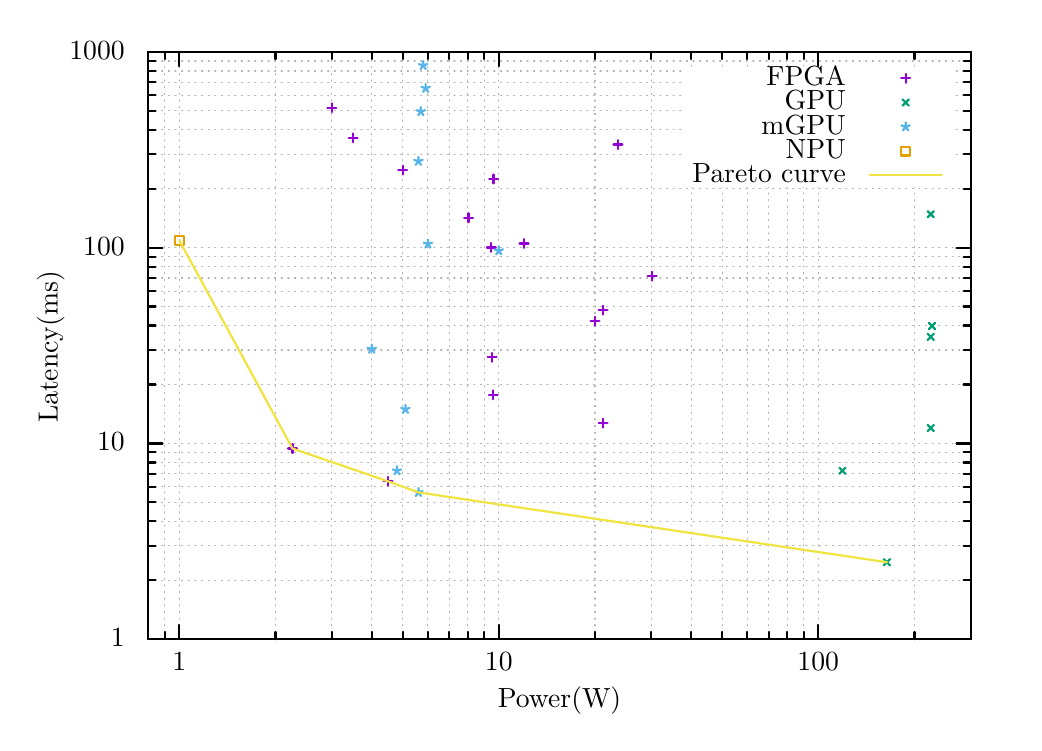
\begin{tikzpicture}[gnuplot]
%% generated with GNUPLOT 5.2p2 (Lua 5.3; terminal rev. 99, script rev. 102)
%% Di 18 Dez 2018 07:50:25 CET
\path (0.000,0.000) rectangle (12.500,8.750);
\gpcolor{color=gp lt color axes}
\gpsetlinetype{gp lt axes}
\gpsetdashtype{gp dt axes}
\gpsetlinewidth{1.00}
\draw[gp path] (1.504,0.985)--(11.947,0.985);
\gpcolor{color=gp lt color border}
\gpsetlinetype{gp lt border}
\gpsetdashtype{gp dt solid}
\gpsetlinewidth{2.00}
\draw[gp path] (1.504,0.985)--(1.684,0.985);
\draw[gp path] (11.947,0.985)--(11.767,0.985);
\node[gp node right] at (1.320,0.985) {$1$};
\gpcolor{color=gp lt color axes}
\gpsetlinetype{gp lt axes}
\gpsetdashtype{gp dt axes}
\gpsetlinewidth{1.00}
\draw[gp path] (1.504,1.733)--(11.947,1.733);
\gpcolor{color=gp lt color border}
\gpsetlinetype{gp lt border}
\gpsetdashtype{gp dt solid}
\gpsetlinewidth{2.00}
\draw[gp path] (1.504,1.733)--(1.594,1.733);
\draw[gp path] (11.947,1.733)--(11.857,1.733);
\gpcolor{color=gp lt color axes}
\gpsetlinetype{gp lt axes}
\gpsetdashtype{gp dt axes}
\gpsetlinewidth{1.00}
\draw[gp path] (1.504,2.171)--(11.947,2.171);
\gpcolor{color=gp lt color border}
\gpsetlinetype{gp lt border}
\gpsetdashtype{gp dt solid}
\gpsetlinewidth{2.00}
\draw[gp path] (1.504,2.171)--(1.594,2.171);
\draw[gp path] (11.947,2.171)--(11.857,2.171);
\gpcolor{color=gp lt color axes}
\gpsetlinetype{gp lt axes}
\gpsetdashtype{gp dt axes}
\gpsetlinewidth{1.00}
\draw[gp path] (1.504,2.481)--(11.947,2.481);
\gpcolor{color=gp lt color border}
\gpsetlinetype{gp lt border}
\gpsetdashtype{gp dt solid}
\gpsetlinewidth{2.00}
\draw[gp path] (1.504,2.481)--(1.594,2.481);
\draw[gp path] (11.947,2.481)--(11.857,2.481);
\gpcolor{color=gp lt color axes}
\gpsetlinetype{gp lt axes}
\gpsetdashtype{gp dt axes}
\gpsetlinewidth{1.00}
\draw[gp path] (1.504,2.722)--(11.947,2.722);
\gpcolor{color=gp lt color border}
\gpsetlinetype{gp lt border}
\gpsetdashtype{gp dt solid}
\gpsetlinewidth{2.00}
\draw[gp path] (1.504,2.722)--(1.594,2.722);
\draw[gp path] (11.947,2.722)--(11.857,2.722);
\gpcolor{color=gp lt color axes}
\gpsetlinetype{gp lt axes}
\gpsetdashtype{gp dt axes}
\gpsetlinewidth{1.00}
\draw[gp path] (1.504,2.919)--(11.947,2.919);
\gpcolor{color=gp lt color border}
\gpsetlinetype{gp lt border}
\gpsetdashtype{gp dt solid}
\gpsetlinewidth{2.00}
\draw[gp path] (1.504,2.919)--(1.594,2.919);
\draw[gp path] (11.947,2.919)--(11.857,2.919);
\gpcolor{color=gp lt color axes}
\gpsetlinetype{gp lt axes}
\gpsetdashtype{gp dt axes}
\gpsetlinewidth{1.00}
\draw[gp path] (1.504,3.085)--(11.947,3.085);
\gpcolor{color=gp lt color border}
\gpsetlinetype{gp lt border}
\gpsetdashtype{gp dt solid}
\gpsetlinewidth{2.00}
\draw[gp path] (1.504,3.085)--(1.594,3.085);
\draw[gp path] (11.947,3.085)--(11.857,3.085);
\gpcolor{color=gp lt color axes}
\gpsetlinetype{gp lt axes}
\gpsetdashtype{gp dt axes}
\gpsetlinewidth{1.00}
\draw[gp path] (1.504,3.229)--(11.947,3.229);
\gpcolor{color=gp lt color border}
\gpsetlinetype{gp lt border}
\gpsetdashtype{gp dt solid}
\gpsetlinewidth{2.00}
\draw[gp path] (1.504,3.229)--(1.594,3.229);
\draw[gp path] (11.947,3.229)--(11.857,3.229);
\gpcolor{color=gp lt color axes}
\gpsetlinetype{gp lt axes}
\gpsetdashtype{gp dt axes}
\gpsetlinewidth{1.00}
\draw[gp path] (1.504,3.357)--(11.947,3.357);
\gpcolor{color=gp lt color border}
\gpsetlinetype{gp lt border}
\gpsetdashtype{gp dt solid}
\gpsetlinewidth{2.00}
\draw[gp path] (1.504,3.357)--(1.594,3.357);
\draw[gp path] (11.947,3.357)--(11.857,3.357);
\gpcolor{color=gp lt color axes}
\gpsetlinetype{gp lt axes}
\gpsetdashtype{gp dt axes}
\gpsetlinewidth{1.00}
\draw[gp path] (1.504,3.470)--(11.947,3.470);
\gpcolor{color=gp lt color border}
\gpsetlinetype{gp lt border}
\gpsetdashtype{gp dt solid}
\gpsetlinewidth{2.00}
\draw[gp path] (1.504,3.470)--(1.684,3.470);
\draw[gp path] (11.947,3.470)--(11.767,3.470);
\node[gp node right] at (1.320,3.470) {$10$};
\gpcolor{color=gp lt color axes}
\gpsetlinetype{gp lt axes}
\gpsetdashtype{gp dt axes}
\gpsetlinewidth{1.00}
\draw[gp path] (1.504,4.218)--(11.947,4.218);
\gpcolor{color=gp lt color border}
\gpsetlinetype{gp lt border}
\gpsetdashtype{gp dt solid}
\gpsetlinewidth{2.00}
\draw[gp path] (1.504,4.218)--(1.594,4.218);
\draw[gp path] (11.947,4.218)--(11.857,4.218);
\gpcolor{color=gp lt color axes}
\gpsetlinetype{gp lt axes}
\gpsetdashtype{gp dt axes}
\gpsetlinewidth{1.00}
\draw[gp path] (1.504,4.656)--(11.947,4.656);
\gpcolor{color=gp lt color border}
\gpsetlinetype{gp lt border}
\gpsetdashtype{gp dt solid}
\gpsetlinewidth{2.00}
\draw[gp path] (1.504,4.656)--(1.594,4.656);
\draw[gp path] (11.947,4.656)--(11.857,4.656);
\gpcolor{color=gp lt color axes}
\gpsetlinetype{gp lt axes}
\gpsetdashtype{gp dt axes}
\gpsetlinewidth{1.00}
\draw[gp path] (1.504,4.967)--(11.947,4.967);
\gpcolor{color=gp lt color border}
\gpsetlinetype{gp lt border}
\gpsetdashtype{gp dt solid}
\gpsetlinewidth{2.00}
\draw[gp path] (1.504,4.967)--(1.594,4.967);
\draw[gp path] (11.947,4.967)--(11.857,4.967);
\gpcolor{color=gp lt color axes}
\gpsetlinetype{gp lt axes}
\gpsetdashtype{gp dt axes}
\gpsetlinewidth{1.00}
\draw[gp path] (1.504,5.208)--(11.947,5.208);
\gpcolor{color=gp lt color border}
\gpsetlinetype{gp lt border}
\gpsetdashtype{gp dt solid}
\gpsetlinewidth{2.00}
\draw[gp path] (1.504,5.208)--(1.594,5.208);
\draw[gp path] (11.947,5.208)--(11.857,5.208);
\gpcolor{color=gp lt color axes}
\gpsetlinetype{gp lt axes}
\gpsetdashtype{gp dt axes}
\gpsetlinewidth{1.00}
\draw[gp path] (1.504,5.404)--(11.947,5.404);
\gpcolor{color=gp lt color border}
\gpsetlinetype{gp lt border}
\gpsetdashtype{gp dt solid}
\gpsetlinewidth{2.00}
\draw[gp path] (1.504,5.404)--(1.594,5.404);
\draw[gp path] (11.947,5.404)--(11.857,5.404);
\gpcolor{color=gp lt color axes}
\gpsetlinetype{gp lt axes}
\gpsetdashtype{gp dt axes}
\gpsetlinewidth{1.00}
\draw[gp path] (1.504,5.571)--(11.947,5.571);
\gpcolor{color=gp lt color border}
\gpsetlinetype{gp lt border}
\gpsetdashtype{gp dt solid}
\gpsetlinewidth{2.00}
\draw[gp path] (1.504,5.571)--(1.594,5.571);
\draw[gp path] (11.947,5.571)--(11.857,5.571);
\gpcolor{color=gp lt color axes}
\gpsetlinetype{gp lt axes}
\gpsetdashtype{gp dt axes}
\gpsetlinewidth{1.00}
\draw[gp path] (1.504,5.715)--(11.947,5.715);
\gpcolor{color=gp lt color border}
\gpsetlinetype{gp lt border}
\gpsetdashtype{gp dt solid}
\gpsetlinewidth{2.00}
\draw[gp path] (1.504,5.715)--(1.594,5.715);
\draw[gp path] (11.947,5.715)--(11.857,5.715);
\gpcolor{color=gp lt color axes}
\gpsetlinetype{gp lt axes}
\gpsetdashtype{gp dt axes}
\gpsetlinewidth{1.00}
\draw[gp path] (1.504,5.842)--(11.947,5.842);
\gpcolor{color=gp lt color border}
\gpsetlinetype{gp lt border}
\gpsetdashtype{gp dt solid}
\gpsetlinewidth{2.00}
\draw[gp path] (1.504,5.842)--(1.594,5.842);
\draw[gp path] (11.947,5.842)--(11.857,5.842);
\gpcolor{color=gp lt color axes}
\gpsetlinetype{gp lt axes}
\gpsetdashtype{gp dt axes}
\gpsetlinewidth{1.00}
\draw[gp path] (1.504,5.956)--(11.947,5.956);
\gpcolor{color=gp lt color border}
\gpsetlinetype{gp lt border}
\gpsetdashtype{gp dt solid}
\gpsetlinewidth{2.00}
\draw[gp path] (1.504,5.956)--(1.684,5.956);
\draw[gp path] (11.947,5.956)--(11.767,5.956);
\node[gp node right] at (1.320,5.956) {$100$};
\gpcolor{color=gp lt color axes}
\gpsetlinetype{gp lt axes}
\gpsetdashtype{gp dt axes}
\gpsetlinewidth{1.00}
\draw[gp path] (1.504,6.704)--(11.947,6.704);
\gpcolor{color=gp lt color border}
\gpsetlinetype{gp lt border}
\gpsetdashtype{gp dt solid}
\gpsetlinewidth{2.00}
\draw[gp path] (1.504,6.704)--(1.594,6.704);
\draw[gp path] (11.947,6.704)--(11.857,6.704);
\gpcolor{color=gp lt color axes}
\gpsetlinetype{gp lt axes}
\gpsetdashtype{gp dt axes}
\gpsetlinewidth{1.00}
\draw[gp path] (1.504,7.141)--(8.271,7.141);
\draw[gp path] (11.763,7.141)--(11.947,7.141);
\gpcolor{color=gp lt color border}
\gpsetlinetype{gp lt border}
\gpsetdashtype{gp dt solid}
\gpsetlinewidth{2.00}
\draw[gp path] (1.504,7.141)--(1.594,7.141);
\draw[gp path] (11.947,7.141)--(11.857,7.141);
\gpcolor{color=gp lt color axes}
\gpsetlinetype{gp lt axes}
\gpsetdashtype{gp dt axes}
\gpsetlinewidth{1.00}
\draw[gp path] (1.504,7.452)--(8.271,7.452);
\draw[gp path] (11.763,7.452)--(11.947,7.452);
\gpcolor{color=gp lt color border}
\gpsetlinetype{gp lt border}
\gpsetdashtype{gp dt solid}
\gpsetlinewidth{2.00}
\draw[gp path] (1.504,7.452)--(1.594,7.452);
\draw[gp path] (11.947,7.452)--(11.857,7.452);
\gpcolor{color=gp lt color axes}
\gpsetlinetype{gp lt axes}
\gpsetdashtype{gp dt axes}
\gpsetlinewidth{1.00}
\draw[gp path] (1.504,7.693)--(8.271,7.693);
\draw[gp path] (11.763,7.693)--(11.947,7.693);
\gpcolor{color=gp lt color border}
\gpsetlinetype{gp lt border}
\gpsetdashtype{gp dt solid}
\gpsetlinewidth{2.00}
\draw[gp path] (1.504,7.693)--(1.594,7.693);
\draw[gp path] (11.947,7.693)--(11.857,7.693);
\gpcolor{color=gp lt color axes}
\gpsetlinetype{gp lt axes}
\gpsetdashtype{gp dt axes}
\gpsetlinewidth{1.00}
\draw[gp path] (1.504,7.890)--(8.271,7.890);
\draw[gp path] (11.763,7.890)--(11.947,7.890);
\gpcolor{color=gp lt color border}
\gpsetlinetype{gp lt border}
\gpsetdashtype{gp dt solid}
\gpsetlinewidth{2.00}
\draw[gp path] (1.504,7.890)--(1.594,7.890);
\draw[gp path] (11.947,7.890)--(11.857,7.890);
\gpcolor{color=gp lt color axes}
\gpsetlinetype{gp lt axes}
\gpsetdashtype{gp dt axes}
\gpsetlinewidth{1.00}
\draw[gp path] (1.504,8.056)--(8.271,8.056);
\draw[gp path] (11.763,8.056)--(11.947,8.056);
\gpcolor{color=gp lt color border}
\gpsetlinetype{gp lt border}
\gpsetdashtype{gp dt solid}
\gpsetlinewidth{2.00}
\draw[gp path] (1.504,8.056)--(1.594,8.056);
\draw[gp path] (11.947,8.056)--(11.857,8.056);
\gpcolor{color=gp lt color axes}
\gpsetlinetype{gp lt axes}
\gpsetdashtype{gp dt axes}
\gpsetlinewidth{1.00}
\draw[gp path] (1.504,8.200)--(8.271,8.200);
\draw[gp path] (11.763,8.200)--(11.947,8.200);
\gpcolor{color=gp lt color border}
\gpsetlinetype{gp lt border}
\gpsetdashtype{gp dt solid}
\gpsetlinewidth{2.00}
\draw[gp path] (1.504,8.200)--(1.594,8.200);
\draw[gp path] (11.947,8.200)--(11.857,8.200);
\gpcolor{color=gp lt color axes}
\gpsetlinetype{gp lt axes}
\gpsetdashtype{gp dt axes}
\gpsetlinewidth{1.00}
\draw[gp path] (1.504,8.327)--(11.947,8.327);
\gpcolor{color=gp lt color border}
\gpsetlinetype{gp lt border}
\gpsetdashtype{gp dt solid}
\gpsetlinewidth{2.00}
\draw[gp path] (1.504,8.327)--(1.594,8.327);
\draw[gp path] (11.947,8.327)--(11.857,8.327);
\gpcolor{color=gp lt color axes}
\gpsetlinetype{gp lt axes}
\gpsetdashtype{gp dt axes}
\gpsetlinewidth{1.00}
\draw[gp path] (1.504,8.441)--(11.947,8.441);
\gpcolor{color=gp lt color border}
\gpsetlinetype{gp lt border}
\gpsetdashtype{gp dt solid}
\gpsetlinewidth{2.00}
\draw[gp path] (1.504,8.441)--(1.684,8.441);
\draw[gp path] (11.947,8.441)--(11.767,8.441);
\node[gp node right] at (1.320,8.441) {$1000$};
\gpcolor{color=gp lt color axes}
\gpsetlinetype{gp lt axes}
\gpsetdashtype{gp dt axes}
\gpsetlinewidth{1.00}
\draw[gp path] (1.504,0.985)--(1.504,8.441);
\gpcolor{color=gp lt color border}
\gpsetlinetype{gp lt border}
\gpsetdashtype{gp dt solid}
\gpsetlinewidth{2.00}
\draw[gp path] (1.504,0.985)--(1.504,1.075);
\draw[gp path] (1.504,8.441)--(1.504,8.351);
\gpcolor{color=gp lt color axes}
\gpsetlinetype{gp lt axes}
\gpsetdashtype{gp dt axes}
\gpsetlinewidth{1.00}
\draw[gp path] (1.712,0.985)--(1.712,8.441);
\gpcolor{color=gp lt color border}
\gpsetlinetype{gp lt border}
\gpsetdashtype{gp dt solid}
\gpsetlinewidth{2.00}
\draw[gp path] (1.712,0.985)--(1.712,1.075);
\draw[gp path] (1.712,8.441)--(1.712,8.351);
\gpcolor{color=gp lt color axes}
\gpsetlinetype{gp lt axes}
\gpsetdashtype{gp dt axes}
\gpsetlinewidth{1.00}
\draw[gp path] (1.897,0.985)--(1.897,8.441);
\gpcolor{color=gp lt color border}
\gpsetlinetype{gp lt border}
\gpsetdashtype{gp dt solid}
\gpsetlinewidth{2.00}
\draw[gp path] (1.897,0.985)--(1.897,1.165);
\draw[gp path] (1.897,8.441)--(1.897,8.261);
\node[gp node center] at (1.897,0.677) {$1$};
\gpcolor{color=gp lt color axes}
\gpsetlinetype{gp lt axes}
\gpsetdashtype{gp dt axes}
\gpsetlinewidth{1.00}
\draw[gp path] (3.118,0.985)--(3.118,8.441);
\gpcolor{color=gp lt color border}
\gpsetlinetype{gp lt border}
\gpsetdashtype{gp dt solid}
\gpsetlinewidth{2.00}
\draw[gp path] (3.118,0.985)--(3.118,1.075);
\draw[gp path] (3.118,8.441)--(3.118,8.351);
\gpcolor{color=gp lt color axes}
\gpsetlinetype{gp lt axes}
\gpsetdashtype{gp dt axes}
\gpsetlinewidth{1.00}
\draw[gp path] (3.833,0.985)--(3.833,8.441);
\gpcolor{color=gp lt color border}
\gpsetlinetype{gp lt border}
\gpsetdashtype{gp dt solid}
\gpsetlinewidth{2.00}
\draw[gp path] (3.833,0.985)--(3.833,1.075);
\draw[gp path] (3.833,8.441)--(3.833,8.351);
\gpcolor{color=gp lt color axes}
\gpsetlinetype{gp lt axes}
\gpsetdashtype{gp dt axes}
\gpsetlinewidth{1.00}
\draw[gp path] (4.340,0.985)--(4.340,8.441);
\gpcolor{color=gp lt color border}
\gpsetlinetype{gp lt border}
\gpsetdashtype{gp dt solid}
\gpsetlinewidth{2.00}
\draw[gp path] (4.340,0.985)--(4.340,1.075);
\draw[gp path] (4.340,8.441)--(4.340,8.351);
\gpcolor{color=gp lt color axes}
\gpsetlinetype{gp lt axes}
\gpsetdashtype{gp dt axes}
\gpsetlinewidth{1.00}
\draw[gp path] (4.733,0.985)--(4.733,8.441);
\gpcolor{color=gp lt color border}
\gpsetlinetype{gp lt border}
\gpsetdashtype{gp dt solid}
\gpsetlinewidth{2.00}
\draw[gp path] (4.733,0.985)--(4.733,1.075);
\draw[gp path] (4.733,8.441)--(4.733,8.351);
\gpcolor{color=gp lt color axes}
\gpsetlinetype{gp lt axes}
\gpsetdashtype{gp dt axes}
\gpsetlinewidth{1.00}
\draw[gp path] (5.054,0.985)--(5.054,8.441);
\gpcolor{color=gp lt color border}
\gpsetlinetype{gp lt border}
\gpsetdashtype{gp dt solid}
\gpsetlinewidth{2.00}
\draw[gp path] (5.054,0.985)--(5.054,1.075);
\draw[gp path] (5.054,8.441)--(5.054,8.351);
\gpcolor{color=gp lt color axes}
\gpsetlinetype{gp lt axes}
\gpsetdashtype{gp dt axes}
\gpsetlinewidth{1.00}
\draw[gp path] (5.326,0.985)--(5.326,8.441);
\gpcolor{color=gp lt color border}
\gpsetlinetype{gp lt border}
\gpsetdashtype{gp dt solid}
\gpsetlinewidth{2.00}
\draw[gp path] (5.326,0.985)--(5.326,1.075);
\draw[gp path] (5.326,8.441)--(5.326,8.351);
\gpcolor{color=gp lt color axes}
\gpsetlinetype{gp lt axes}
\gpsetdashtype{gp dt axes}
\gpsetlinewidth{1.00}
\draw[gp path] (5.561,0.985)--(5.561,8.441);
\gpcolor{color=gp lt color border}
\gpsetlinetype{gp lt border}
\gpsetdashtype{gp dt solid}
\gpsetlinewidth{2.00}
\draw[gp path] (5.561,0.985)--(5.561,1.075);
\draw[gp path] (5.561,8.441)--(5.561,8.351);
\gpcolor{color=gp lt color axes}
\gpsetlinetype{gp lt axes}
\gpsetdashtype{gp dt axes}
\gpsetlinewidth{1.00}
\draw[gp path] (5.769,0.985)--(5.769,8.441);
\gpcolor{color=gp lt color border}
\gpsetlinetype{gp lt border}
\gpsetdashtype{gp dt solid}
\gpsetlinewidth{2.00}
\draw[gp path] (5.769,0.985)--(5.769,1.075);
\draw[gp path] (5.769,8.441)--(5.769,8.351);
\gpcolor{color=gp lt color axes}
\gpsetlinetype{gp lt axes}
\gpsetdashtype{gp dt axes}
\gpsetlinewidth{1.00}
\draw[gp path] (5.954,0.985)--(5.954,8.441);
\gpcolor{color=gp lt color border}
\gpsetlinetype{gp lt border}
\gpsetdashtype{gp dt solid}
\gpsetlinewidth{2.00}
\draw[gp path] (5.954,0.985)--(5.954,1.165);
\draw[gp path] (5.954,8.441)--(5.954,8.261);
\node[gp node center] at (5.954,0.677) {$10$};
\gpcolor{color=gp lt color axes}
\gpsetlinetype{gp lt axes}
\gpsetdashtype{gp dt axes}
\gpsetlinewidth{1.00}
\draw[gp path] (7.176,0.985)--(7.176,8.441);
\gpcolor{color=gp lt color border}
\gpsetlinetype{gp lt border}
\gpsetdashtype{gp dt solid}
\gpsetlinewidth{2.00}
\draw[gp path] (7.176,0.985)--(7.176,1.075);
\draw[gp path] (7.176,8.441)--(7.176,8.351);
\gpcolor{color=gp lt color axes}
\gpsetlinetype{gp lt axes}
\gpsetdashtype{gp dt axes}
\gpsetlinewidth{1.00}
\draw[gp path] (7.890,0.985)--(7.890,8.441);
\gpcolor{color=gp lt color border}
\gpsetlinetype{gp lt border}
\gpsetdashtype{gp dt solid}
\gpsetlinewidth{2.00}
\draw[gp path] (7.890,0.985)--(7.890,1.075);
\draw[gp path] (7.890,8.441)--(7.890,8.351);
\gpcolor{color=gp lt color axes}
\gpsetlinetype{gp lt axes}
\gpsetdashtype{gp dt axes}
\gpsetlinewidth{1.00}
\draw[gp path] (8.397,0.985)--(8.397,6.721);
\draw[gp path] (8.397,8.261)--(8.397,8.441);
\gpcolor{color=gp lt color border}
\gpsetlinetype{gp lt border}
\gpsetdashtype{gp dt solid}
\gpsetlinewidth{2.00}
\draw[gp path] (8.397,0.985)--(8.397,1.075);
\draw[gp path] (8.397,8.441)--(8.397,8.351);
\gpcolor{color=gp lt color axes}
\gpsetlinetype{gp lt axes}
\gpsetdashtype{gp dt axes}
\gpsetlinewidth{1.00}
\draw[gp path] (8.790,0.985)--(8.790,6.721);
\draw[gp path] (8.790,8.261)--(8.790,8.441);
\gpcolor{color=gp lt color border}
\gpsetlinetype{gp lt border}
\gpsetdashtype{gp dt solid}
\gpsetlinewidth{2.00}
\draw[gp path] (8.790,0.985)--(8.790,1.075);
\draw[gp path] (8.790,8.441)--(8.790,8.351);
\gpcolor{color=gp lt color axes}
\gpsetlinetype{gp lt axes}
\gpsetdashtype{gp dt axes}
\gpsetlinewidth{1.00}
\draw[gp path] (9.111,0.985)--(9.111,6.721);
\draw[gp path] (9.111,8.261)--(9.111,8.441);
\gpcolor{color=gp lt color border}
\gpsetlinetype{gp lt border}
\gpsetdashtype{gp dt solid}
\gpsetlinewidth{2.00}
\draw[gp path] (9.111,0.985)--(9.111,1.075);
\draw[gp path] (9.111,8.441)--(9.111,8.351);
\gpcolor{color=gp lt color axes}
\gpsetlinetype{gp lt axes}
\gpsetdashtype{gp dt axes}
\gpsetlinewidth{1.00}
\draw[gp path] (9.383,0.985)--(9.383,6.721);
\draw[gp path] (9.383,8.261)--(9.383,8.441);
\gpcolor{color=gp lt color border}
\gpsetlinetype{gp lt border}
\gpsetdashtype{gp dt solid}
\gpsetlinewidth{2.00}
\draw[gp path] (9.383,0.985)--(9.383,1.075);
\draw[gp path] (9.383,8.441)--(9.383,8.351);
\gpcolor{color=gp lt color axes}
\gpsetlinetype{gp lt axes}
\gpsetdashtype{gp dt axes}
\gpsetlinewidth{1.00}
\draw[gp path] (9.618,0.985)--(9.618,6.721);
\draw[gp path] (9.618,8.261)--(9.618,8.441);
\gpcolor{color=gp lt color border}
\gpsetlinetype{gp lt border}
\gpsetdashtype{gp dt solid}
\gpsetlinewidth{2.00}
\draw[gp path] (9.618,0.985)--(9.618,1.075);
\draw[gp path] (9.618,8.441)--(9.618,8.351);
\gpcolor{color=gp lt color axes}
\gpsetlinetype{gp lt axes}
\gpsetdashtype{gp dt axes}
\gpsetlinewidth{1.00}
\draw[gp path] (9.826,0.985)--(9.826,6.721);
\draw[gp path] (9.826,8.261)--(9.826,8.441);
\gpcolor{color=gp lt color border}
\gpsetlinetype{gp lt border}
\gpsetdashtype{gp dt solid}
\gpsetlinewidth{2.00}
\draw[gp path] (9.826,0.985)--(9.826,1.075);
\draw[gp path] (9.826,8.441)--(9.826,8.351);
\gpcolor{color=gp lt color axes}
\gpsetlinetype{gp lt axes}
\gpsetdashtype{gp dt axes}
\gpsetlinewidth{1.00}
\draw[gp path] (10.011,0.985)--(10.011,6.721);
\draw[gp path] (10.011,8.261)--(10.011,8.441);
\gpcolor{color=gp lt color border}
\gpsetlinetype{gp lt border}
\gpsetdashtype{gp dt solid}
\gpsetlinewidth{2.00}
\draw[gp path] (10.011,0.985)--(10.011,1.165);
\draw[gp path] (10.011,8.441)--(10.011,8.261);
\node[gp node center] at (10.011,0.677) {$100$};
\gpcolor{color=gp lt color axes}
\gpsetlinetype{gp lt axes}
\gpsetdashtype{gp dt axes}
\gpsetlinewidth{1.00}
\draw[gp path] (11.233,0.985)--(11.233,6.721);
\draw[gp path] (11.233,8.261)--(11.233,8.441);
\gpcolor{color=gp lt color border}
\gpsetlinetype{gp lt border}
\gpsetdashtype{gp dt solid}
\gpsetlinewidth{2.00}
\draw[gp path] (11.233,0.985)--(11.233,1.075);
\draw[gp path] (11.233,8.441)--(11.233,8.351);
\gpcolor{color=gp lt color axes}
\gpsetlinetype{gp lt axes}
\gpsetdashtype{gp dt axes}
\gpsetlinewidth{1.00}
\draw[gp path] (11.947,0.985)--(11.947,8.441);
\gpcolor{color=gp lt color border}
\gpsetlinetype{gp lt border}
\gpsetdashtype{gp dt solid}
\gpsetlinewidth{2.00}
\draw[gp path] (11.947,0.985)--(11.947,1.075);
\draw[gp path] (11.947,8.441)--(11.947,8.351);
\draw[gp path] (1.504,8.441)--(1.504,0.985)--(11.947,0.985)--(11.947,8.441)--cycle;
\node[gp node center,rotate=-270] at (0.276,4.713) {Latency(ms)};
\node[gp node center] at (6.725,0.215) {Power(W)};
\node[gp node right] at (10.479,8.107) {FPGA};
\gpcolor{rgb color={0.580,0.000,0.827}}
\gpsetpointsize{4.00}
\gppoint{gp mark 1}{(3.334,3.405)}
\gppoint{gp mark 1}{(7.467,7.265)}
\gppoint{gp mark 1}{(5.888,6.829)}
\gppoint{gp mark 1}{(7.902,5.595)}
\gppoint{gp mark 1}{(7.278,5.163)}
\gppoint{gp mark 1}{(7.278,3.728)}
\gppoint{gp mark 1}{(5.570,6.336)}
\gppoint{gp mark 1}{(7.176,5.022)}
\gppoint{gp mark 1}{(4.104,7.350)}
\gppoint{gp mark 1}{(4.733,6.942)}
\gppoint{gp mark 1}{(5.869,4.564)}
\gppoint{gp mark 1}{(5.884,4.087)}
\gppoint{gp mark 1}{(5.860,5.959)}
\gppoint{gp mark 1}{(3.833,7.733)}
\gppoint{gp mark 1}{(6.275,6.009)}
\gppoint{gp mark 1}{(4.547,2.989)}
\gppoint{gp mark 1}{(11.121,8.107)}
\gpcolor{color=gp lt color border}
\node[gp node right] at (10.479,7.799) {GPU};
\gpcolor{rgb color={0.000,0.620,0.451}}
\gppoint{gp mark 2}{(10.883,1.961)}
\gppoint{gp mark 2}{(11.456,4.961)}
\gppoint{gp mark 2}{(11.440,3.665)}
\gppoint{gp mark 2}{(10.318,3.123)}
\gppoint{gp mark 2}{(11.440,6.381)}
\gppoint{gp mark 2}{(11.440,4.823)}
\gppoint{gp mark 2}{(11.121,7.799)}
\gpcolor{color=gp lt color border}
\node[gp node right] at (10.479,7.491) {mGPU};
\gpcolor{rgb color={0.337,0.706,0.914}}
\gppoint{gp mark 3}{(5.954,5.917)}
\gppoint{gp mark 3}{(4.768,3.903)}
\gppoint{gp mark 3}{(4.964,7.684)}
\gppoint{gp mark 3}{(4.933,2.848)}
\gppoint{gp mark 3}{(4.933,7.053)}
\gppoint{gp mark 3}{(4.340,4.667)}
\gppoint{gp mark 3}{(4.994,8.270)}
\gppoint{gp mark 3}{(4.661,3.123)}
\gppoint{gp mark 3}{(5.025,7.981)}
\gppoint{gp mark 3}{(5.054,6.002)}
\gppoint{gp mark 3}{(11.121,7.491)}
\gpcolor{color=gp lt color border}
\node[gp node right] at (10.479,7.183) {NPU};
\gpcolor{rgb color={0.902,0.624,0.000}}
\gppoint{gp mark 4}{(1.897,6.048)}
\gppoint{gp mark 4}{(11.121,7.183)}
\gpcolor{color=gp lt color border}
\node[gp node right] at (10.479,6.875) {Pareto curve};
\gpcolor{rgb color={0.941,0.894,0.259}}
\draw[gp path] (10.663,6.875)--(11.579,6.875);
\draw[gp path] (1.897,6.048)--(3.334,3.405)--(4.547,2.989)--(4.933,2.848)--(10.883,1.961);
\gpcolor{color=gp lt color border}
\draw[gp path] (1.504,8.441)--(1.504,0.985)--(11.947,0.985)--(11.947,8.441)--cycle;
%% coordinates of the plot area
\gpdefrectangularnode{gp plot 1}{\pgfpoint{1.504cm}{0.985cm}}{\pgfpoint{11.947cm}{8.441cm}}
\end{tikzpicture}
%% gnuplot variables
}
    \hfill
    \scalebox{0.8}{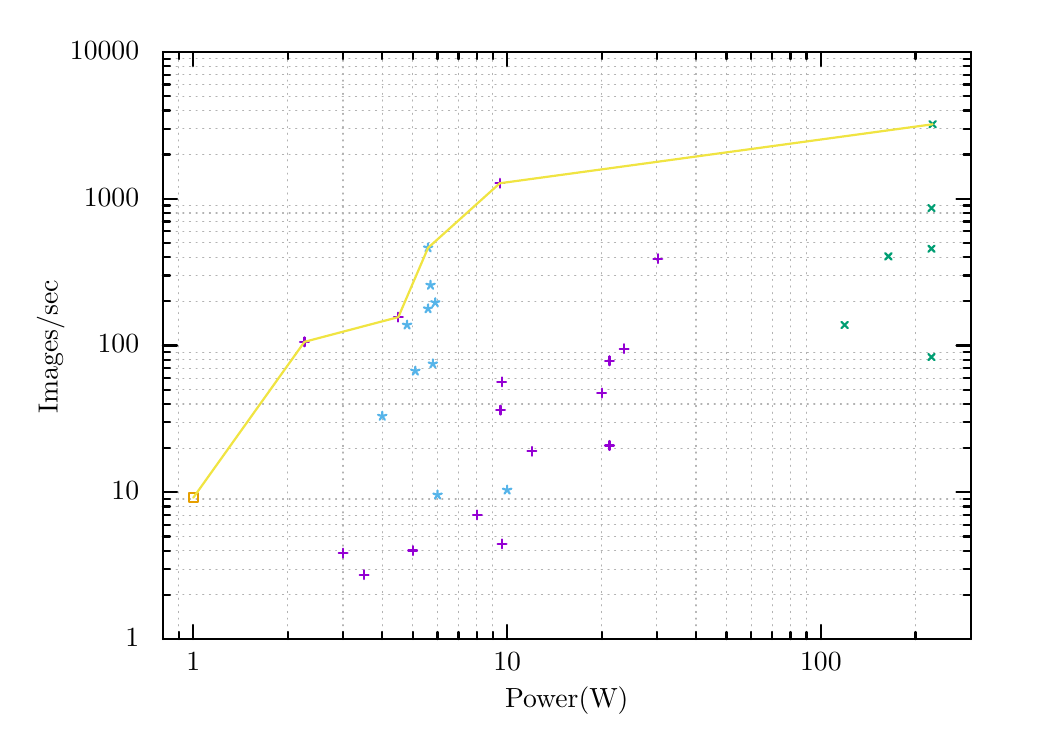
\begin{tikzpicture}[gnuplot]
%% generated with GNUPLOT 5.2p2 (Lua 5.3; terminal rev. 99, script rev. 102)
%% Di 18 Dez 2018 07:10:48 CET
\path (0.000,0.000) rectangle (12.500,8.750);
\gpcolor{color=gp lt color border}
\gpsetlinetype{gp lt border}
\gpsetdashtype{gp dt solid}
\gpsetlinewidth{2.00}
\draw[gp path] (1.688,0.985)--(1.868,0.985);
\draw[gp path] (11.947,0.985)--(11.767,0.985);
\node[gp node right] at (1.504,0.985) {$1$};
\gpcolor{color=gp lt color axes}
\gpsetlinetype{gp lt axes}
\gpsetdashtype{gp dt axes}
\gpsetlinewidth{1.00}
\draw[gp path] (1.688,1.546)--(11.947,1.546);
\gpcolor{color=gp lt color border}
\gpsetlinetype{gp lt border}
\gpsetdashtype{gp dt solid}
\gpsetlinewidth{2.00}
\draw[gp path] (1.688,1.546)--(1.778,1.546);
\draw[gp path] (11.947,1.546)--(11.857,1.546);
\gpcolor{color=gp lt color axes}
\gpsetlinetype{gp lt axes}
\gpsetdashtype{gp dt axes}
\gpsetlinewidth{1.00}
\draw[gp path] (1.688,1.874)--(11.947,1.874);
\gpcolor{color=gp lt color border}
\gpsetlinetype{gp lt border}
\gpsetdashtype{gp dt solid}
\gpsetlinewidth{2.00}
\draw[gp path] (1.688,1.874)--(1.778,1.874);
\draw[gp path] (11.947,1.874)--(11.857,1.874);
\gpcolor{color=gp lt color axes}
\gpsetlinetype{gp lt axes}
\gpsetdashtype{gp dt axes}
\gpsetlinewidth{1.00}
\draw[gp path] (1.688,2.107)--(11.947,2.107);
\gpcolor{color=gp lt color border}
\gpsetlinetype{gp lt border}
\gpsetdashtype{gp dt solid}
\gpsetlinewidth{2.00}
\draw[gp path] (1.688,2.107)--(1.778,2.107);
\draw[gp path] (11.947,2.107)--(11.857,2.107);
\gpcolor{color=gp lt color axes}
\gpsetlinetype{gp lt axes}
\gpsetdashtype{gp dt axes}
\gpsetlinewidth{1.00}
\draw[gp path] (1.688,2.288)--(11.947,2.288);
\gpcolor{color=gp lt color border}
\gpsetlinetype{gp lt border}
\gpsetdashtype{gp dt solid}
\gpsetlinewidth{2.00}
\draw[gp path] (1.688,2.288)--(1.778,2.288);
\draw[gp path] (11.947,2.288)--(11.857,2.288);
\gpcolor{color=gp lt color axes}
\gpsetlinetype{gp lt axes}
\gpsetdashtype{gp dt axes}
\gpsetlinewidth{1.00}
\draw[gp path] (1.688,2.435)--(11.947,2.435);
\gpcolor{color=gp lt color border}
\gpsetlinetype{gp lt border}
\gpsetdashtype{gp dt solid}
\gpsetlinewidth{2.00}
\draw[gp path] (1.688,2.435)--(1.778,2.435);
\draw[gp path] (11.947,2.435)--(11.857,2.435);
\gpcolor{color=gp lt color axes}
\gpsetlinetype{gp lt axes}
\gpsetdashtype{gp dt axes}
\gpsetlinewidth{1.00}
\draw[gp path] (1.688,2.560)--(11.947,2.560);
\gpcolor{color=gp lt color border}
\gpsetlinetype{gp lt border}
\gpsetdashtype{gp dt solid}
\gpsetlinewidth{2.00}
\draw[gp path] (1.688,2.560)--(1.778,2.560);
\draw[gp path] (11.947,2.560)--(11.857,2.560);
\gpcolor{color=gp lt color axes}
\gpsetlinetype{gp lt axes}
\gpsetdashtype{gp dt axes}
\gpsetlinewidth{1.00}
\draw[gp path] (1.688,2.668)--(11.947,2.668);
\gpcolor{color=gp lt color border}
\gpsetlinetype{gp lt border}
\gpsetdashtype{gp dt solid}
\gpsetlinewidth{2.00}
\draw[gp path] (1.688,2.668)--(1.778,2.668);
\draw[gp path] (11.947,2.668)--(11.857,2.668);
\gpcolor{color=gp lt color axes}
\gpsetlinetype{gp lt axes}
\gpsetdashtype{gp dt axes}
\gpsetlinewidth{1.00}
\draw[gp path] (1.688,2.764)--(11.947,2.764);
\gpcolor{color=gp lt color border}
\gpsetlinetype{gp lt border}
\gpsetdashtype{gp dt solid}
\gpsetlinewidth{2.00}
\draw[gp path] (1.688,2.764)--(1.778,2.764);
\draw[gp path] (11.947,2.764)--(11.857,2.764);
\draw[gp path] (1.688,2.849)--(1.868,2.849);
\draw[gp path] (11.947,2.849)--(11.767,2.849);
\node[gp node right] at (1.504,2.849) {$10$};
\gpcolor{color=gp lt color axes}
\gpsetlinetype{gp lt axes}
\gpsetdashtype{gp dt axes}
\gpsetlinewidth{1.00}
\draw[gp path] (1.688,3.410)--(11.947,3.410);
\gpcolor{color=gp lt color border}
\gpsetlinetype{gp lt border}
\gpsetdashtype{gp dt solid}
\gpsetlinewidth{2.00}
\draw[gp path] (1.688,3.410)--(1.778,3.410);
\draw[gp path] (11.947,3.410)--(11.857,3.410);
\gpcolor{color=gp lt color axes}
\gpsetlinetype{gp lt axes}
\gpsetdashtype{gp dt axes}
\gpsetlinewidth{1.00}
\draw[gp path] (1.688,3.738)--(11.947,3.738);
\gpcolor{color=gp lt color border}
\gpsetlinetype{gp lt border}
\gpsetdashtype{gp dt solid}
\gpsetlinewidth{2.00}
\draw[gp path] (1.688,3.738)--(1.778,3.738);
\draw[gp path] (11.947,3.738)--(11.857,3.738);
\gpcolor{color=gp lt color axes}
\gpsetlinetype{gp lt axes}
\gpsetdashtype{gp dt axes}
\gpsetlinewidth{1.00}
\draw[gp path] (1.688,3.971)--(11.947,3.971);
\gpcolor{color=gp lt color border}
\gpsetlinetype{gp lt border}
\gpsetdashtype{gp dt solid}
\gpsetlinewidth{2.00}
\draw[gp path] (1.688,3.971)--(1.778,3.971);
\draw[gp path] (11.947,3.971)--(11.857,3.971);
\gpcolor{color=gp lt color axes}
\gpsetlinetype{gp lt axes}
\gpsetdashtype{gp dt axes}
\gpsetlinewidth{1.00}
\draw[gp path] (1.688,4.152)--(11.947,4.152);
\gpcolor{color=gp lt color border}
\gpsetlinetype{gp lt border}
\gpsetdashtype{gp dt solid}
\gpsetlinewidth{2.00}
\draw[gp path] (1.688,4.152)--(1.778,4.152);
\draw[gp path] (11.947,4.152)--(11.857,4.152);
\gpcolor{color=gp lt color axes}
\gpsetlinetype{gp lt axes}
\gpsetdashtype{gp dt axes}
\gpsetlinewidth{1.00}
\draw[gp path] (1.688,4.299)--(11.947,4.299);
\gpcolor{color=gp lt color border}
\gpsetlinetype{gp lt border}
\gpsetdashtype{gp dt solid}
\gpsetlinewidth{2.00}
\draw[gp path] (1.688,4.299)--(1.778,4.299);
\draw[gp path] (11.947,4.299)--(11.857,4.299);
\gpcolor{color=gp lt color axes}
\gpsetlinetype{gp lt axes}
\gpsetdashtype{gp dt axes}
\gpsetlinewidth{1.00}
\draw[gp path] (1.688,4.424)--(11.947,4.424);
\gpcolor{color=gp lt color border}
\gpsetlinetype{gp lt border}
\gpsetdashtype{gp dt solid}
\gpsetlinewidth{2.00}
\draw[gp path] (1.688,4.424)--(1.778,4.424);
\draw[gp path] (11.947,4.424)--(11.857,4.424);
\gpcolor{color=gp lt color axes}
\gpsetlinetype{gp lt axes}
\gpsetdashtype{gp dt axes}
\gpsetlinewidth{1.00}
\draw[gp path] (1.688,4.532)--(11.947,4.532);
\gpcolor{color=gp lt color border}
\gpsetlinetype{gp lt border}
\gpsetdashtype{gp dt solid}
\gpsetlinewidth{2.00}
\draw[gp path] (1.688,4.532)--(1.778,4.532);
\draw[gp path] (11.947,4.532)--(11.857,4.532);
\gpcolor{color=gp lt color axes}
\gpsetlinetype{gp lt axes}
\gpsetdashtype{gp dt axes}
\gpsetlinewidth{1.00}
\draw[gp path] (1.688,4.628)--(11.947,4.628);
\gpcolor{color=gp lt color border}
\gpsetlinetype{gp lt border}
\gpsetdashtype{gp dt solid}
\gpsetlinewidth{2.00}
\draw[gp path] (1.688,4.628)--(1.778,4.628);
\draw[gp path] (11.947,4.628)--(11.857,4.628);
\draw[gp path] (1.688,4.713)--(1.868,4.713);
\draw[gp path] (11.947,4.713)--(11.767,4.713);
\node[gp node right] at (1.504,4.713) {$100$};
\gpcolor{color=gp lt color axes}
\gpsetlinetype{gp lt axes}
\gpsetdashtype{gp dt axes}
\gpsetlinewidth{1.00}
\draw[gp path] (1.688,5.274)--(11.947,5.274);
\gpcolor{color=gp lt color border}
\gpsetlinetype{gp lt border}
\gpsetdashtype{gp dt solid}
\gpsetlinewidth{2.00}
\draw[gp path] (1.688,5.274)--(1.778,5.274);
\draw[gp path] (11.947,5.274)--(11.857,5.274);
\gpcolor{color=gp lt color axes}
\gpsetlinetype{gp lt axes}
\gpsetdashtype{gp dt axes}
\gpsetlinewidth{1.00}
\draw[gp path] (1.688,5.602)--(11.947,5.602);
\gpcolor{color=gp lt color border}
\gpsetlinetype{gp lt border}
\gpsetdashtype{gp dt solid}
\gpsetlinewidth{2.00}
\draw[gp path] (1.688,5.602)--(1.778,5.602);
\draw[gp path] (11.947,5.602)--(11.857,5.602);
\gpcolor{color=gp lt color axes}
\gpsetlinetype{gp lt axes}
\gpsetdashtype{gp dt axes}
\gpsetlinewidth{1.00}
\draw[gp path] (1.688,5.835)--(11.947,5.835);
\gpcolor{color=gp lt color border}
\gpsetlinetype{gp lt border}
\gpsetdashtype{gp dt solid}
\gpsetlinewidth{2.00}
\draw[gp path] (1.688,5.835)--(1.778,5.835);
\draw[gp path] (11.947,5.835)--(11.857,5.835);
\gpcolor{color=gp lt color axes}
\gpsetlinetype{gp lt axes}
\gpsetdashtype{gp dt axes}
\gpsetlinewidth{1.00}
\draw[gp path] (1.688,6.016)--(11.947,6.016);
\gpcolor{color=gp lt color border}
\gpsetlinetype{gp lt border}
\gpsetdashtype{gp dt solid}
\gpsetlinewidth{2.00}
\draw[gp path] (1.688,6.016)--(1.778,6.016);
\draw[gp path] (11.947,6.016)--(11.857,6.016);
\gpcolor{color=gp lt color axes}
\gpsetlinetype{gp lt axes}
\gpsetdashtype{gp dt axes}
\gpsetlinewidth{1.00}
\draw[gp path] (1.688,6.163)--(11.947,6.163);
\gpcolor{color=gp lt color border}
\gpsetlinetype{gp lt border}
\gpsetdashtype{gp dt solid}
\gpsetlinewidth{2.00}
\draw[gp path] (1.688,6.163)--(1.778,6.163);
\draw[gp path] (11.947,6.163)--(11.857,6.163);
\gpcolor{color=gp lt color axes}
\gpsetlinetype{gp lt axes}
\gpsetdashtype{gp dt axes}
\gpsetlinewidth{1.00}
\draw[gp path] (1.688,6.288)--(11.947,6.288);
\gpcolor{color=gp lt color border}
\gpsetlinetype{gp lt border}
\gpsetdashtype{gp dt solid}
\gpsetlinewidth{2.00}
\draw[gp path] (1.688,6.288)--(1.778,6.288);
\draw[gp path] (11.947,6.288)--(11.857,6.288);
\gpcolor{color=gp lt color axes}
\gpsetlinetype{gp lt axes}
\gpsetdashtype{gp dt axes}
\gpsetlinewidth{1.00}
\draw[gp path] (1.688,6.396)--(11.947,6.396);
\gpcolor{color=gp lt color border}
\gpsetlinetype{gp lt border}
\gpsetdashtype{gp dt solid}
\gpsetlinewidth{2.00}
\draw[gp path] (1.688,6.396)--(1.778,6.396);
\draw[gp path] (11.947,6.396)--(11.857,6.396);
\gpcolor{color=gp lt color axes}
\gpsetlinetype{gp lt axes}
\gpsetdashtype{gp dt axes}
\gpsetlinewidth{1.00}
\draw[gp path] (1.688,6.492)--(11.947,6.492);
\gpcolor{color=gp lt color border}
\gpsetlinetype{gp lt border}
\gpsetdashtype{gp dt solid}
\gpsetlinewidth{2.00}
\draw[gp path] (1.688,6.492)--(1.778,6.492);
\draw[gp path] (11.947,6.492)--(11.857,6.492);
\draw[gp path] (1.688,6.577)--(1.868,6.577);
\draw[gp path] (11.947,6.577)--(11.767,6.577);
\node[gp node right] at (1.504,6.577) {$1000$};
\gpcolor{color=gp lt color axes}
\gpsetlinetype{gp lt axes}
\gpsetdashtype{gp dt axes}
\gpsetlinewidth{1.00}
\draw[gp path] (1.688,7.138)--(11.947,7.138);
\gpcolor{color=gp lt color border}
\gpsetlinetype{gp lt border}
\gpsetdashtype{gp dt solid}
\gpsetlinewidth{2.00}
\draw[gp path] (1.688,7.138)--(1.778,7.138);
\draw[gp path] (11.947,7.138)--(11.857,7.138);
\gpcolor{color=gp lt color axes}
\gpsetlinetype{gp lt axes}
\gpsetdashtype{gp dt axes}
\gpsetlinewidth{1.00}
\draw[gp path] (1.688,7.466)--(11.947,7.466);
\gpcolor{color=gp lt color border}
\gpsetlinetype{gp lt border}
\gpsetdashtype{gp dt solid}
\gpsetlinewidth{2.00}
\draw[gp path] (1.688,7.466)--(1.778,7.466);
\draw[gp path] (11.947,7.466)--(11.857,7.466);
\gpcolor{color=gp lt color axes}
\gpsetlinetype{gp lt axes}
\gpsetdashtype{gp dt axes}
\gpsetlinewidth{1.00}
\draw[gp path] (1.688,7.699)--(11.947,7.699);
\gpcolor{color=gp lt color border}
\gpsetlinetype{gp lt border}
\gpsetdashtype{gp dt solid}
\gpsetlinewidth{2.00}
\draw[gp path] (1.688,7.699)--(1.778,7.699);
\draw[gp path] (11.947,7.699)--(11.857,7.699);
\gpcolor{color=gp lt color axes}
\gpsetlinetype{gp lt axes}
\gpsetdashtype{gp dt axes}
\gpsetlinewidth{1.00}
\draw[gp path] (1.688,7.880)--(11.947,7.880);
\gpcolor{color=gp lt color border}
\gpsetlinetype{gp lt border}
\gpsetdashtype{gp dt solid}
\gpsetlinewidth{2.00}
\draw[gp path] (1.688,7.880)--(1.778,7.880);
\draw[gp path] (11.947,7.880)--(11.857,7.880);
\gpcolor{color=gp lt color axes}
\gpsetlinetype{gp lt axes}
\gpsetdashtype{gp dt axes}
\gpsetlinewidth{1.00}
\draw[gp path] (1.688,8.027)--(11.947,8.027);
\gpcolor{color=gp lt color border}
\gpsetlinetype{gp lt border}
\gpsetdashtype{gp dt solid}
\gpsetlinewidth{2.00}
\draw[gp path] (1.688,8.027)--(1.778,8.027);
\draw[gp path] (11.947,8.027)--(11.857,8.027);
\gpcolor{color=gp lt color axes}
\gpsetlinetype{gp lt axes}
\gpsetdashtype{gp dt axes}
\gpsetlinewidth{1.00}
\draw[gp path] (1.688,8.152)--(11.947,8.152);
\gpcolor{color=gp lt color border}
\gpsetlinetype{gp lt border}
\gpsetdashtype{gp dt solid}
\gpsetlinewidth{2.00}
\draw[gp path] (1.688,8.152)--(1.778,8.152);
\draw[gp path] (11.947,8.152)--(11.857,8.152);
\gpcolor{color=gp lt color axes}
\gpsetlinetype{gp lt axes}
\gpsetdashtype{gp dt axes}
\gpsetlinewidth{1.00}
\draw[gp path] (1.688,8.260)--(11.947,8.260);
\gpcolor{color=gp lt color border}
\gpsetlinetype{gp lt border}
\gpsetdashtype{gp dt solid}
\gpsetlinewidth{2.00}
\draw[gp path] (1.688,8.260)--(1.778,8.260);
\draw[gp path] (11.947,8.260)--(11.857,8.260);
\gpcolor{color=gp lt color axes}
\gpsetlinetype{gp lt axes}
\gpsetdashtype{gp dt axes}
\gpsetlinewidth{1.00}
\draw[gp path] (1.688,8.356)--(11.947,8.356);
\gpcolor{color=gp lt color border}
\gpsetlinetype{gp lt border}
\gpsetdashtype{gp dt solid}
\gpsetlinewidth{2.00}
\draw[gp path] (1.688,8.356)--(1.778,8.356);
\draw[gp path] (11.947,8.356)--(11.857,8.356);
\draw[gp path] (1.688,8.441)--(1.868,8.441);
\draw[gp path] (11.947,8.441)--(11.767,8.441);
\node[gp node right] at (1.504,8.441) {$10000$};
\gpcolor{color=gp lt color axes}
\gpsetlinetype{gp lt axes}
\gpsetdashtype{gp dt axes}
\gpsetlinewidth{1.00}
\draw[gp path] (1.688,0.985)--(1.688,8.441);
\gpcolor{color=gp lt color border}
\gpsetlinetype{gp lt border}
\gpsetdashtype{gp dt solid}
\gpsetlinewidth{2.00}
\draw[gp path] (1.688,0.985)--(1.688,1.075);
\draw[gp path] (1.688,8.441)--(1.688,8.351);
\gpcolor{color=gp lt color axes}
\gpsetlinetype{gp lt axes}
\gpsetdashtype{gp dt axes}
\gpsetlinewidth{1.00}
\draw[gp path] (1.892,0.985)--(1.892,8.441);
\gpcolor{color=gp lt color border}
\gpsetlinetype{gp lt border}
\gpsetdashtype{gp dt solid}
\gpsetlinewidth{2.00}
\draw[gp path] (1.892,0.985)--(1.892,1.075);
\draw[gp path] (1.892,8.441)--(1.892,8.351);
\draw[gp path] (2.074,0.985)--(2.074,1.165);
\draw[gp path] (2.074,8.441)--(2.074,8.261);
\node[gp node center] at (2.074,0.677) {$1$};
\gpcolor{color=gp lt color axes}
\gpsetlinetype{gp lt axes}
\gpsetdashtype{gp dt axes}
\gpsetlinewidth{1.00}
\draw[gp path] (3.274,0.985)--(3.274,8.441);
\gpcolor{color=gp lt color border}
\gpsetlinetype{gp lt border}
\gpsetdashtype{gp dt solid}
\gpsetlinewidth{2.00}
\draw[gp path] (3.274,0.985)--(3.274,1.075);
\draw[gp path] (3.274,8.441)--(3.274,8.351);
\gpcolor{color=gp lt color axes}
\gpsetlinetype{gp lt axes}
\gpsetdashtype{gp dt axes}
\gpsetlinewidth{1.00}
\draw[gp path] (3.976,0.985)--(3.976,8.441);
\gpcolor{color=gp lt color border}
\gpsetlinetype{gp lt border}
\gpsetdashtype{gp dt solid}
\gpsetlinewidth{2.00}
\draw[gp path] (3.976,0.985)--(3.976,1.075);
\draw[gp path] (3.976,8.441)--(3.976,8.351);
\gpcolor{color=gp lt color axes}
\gpsetlinetype{gp lt axes}
\gpsetdashtype{gp dt axes}
\gpsetlinewidth{1.00}
\draw[gp path] (4.474,0.985)--(4.474,8.441);
\gpcolor{color=gp lt color border}
\gpsetlinetype{gp lt border}
\gpsetdashtype{gp dt solid}
\gpsetlinewidth{2.00}
\draw[gp path] (4.474,0.985)--(4.474,1.075);
\draw[gp path] (4.474,8.441)--(4.474,8.351);
\gpcolor{color=gp lt color axes}
\gpsetlinetype{gp lt axes}
\gpsetdashtype{gp dt axes}
\gpsetlinewidth{1.00}
\draw[gp path] (4.860,0.985)--(4.860,8.441);
\gpcolor{color=gp lt color border}
\gpsetlinetype{gp lt border}
\gpsetdashtype{gp dt solid}
\gpsetlinewidth{2.00}
\draw[gp path] (4.860,0.985)--(4.860,1.075);
\draw[gp path] (4.860,8.441)--(4.860,8.351);
\gpcolor{color=gp lt color axes}
\gpsetlinetype{gp lt axes}
\gpsetdashtype{gp dt axes}
\gpsetlinewidth{1.00}
\draw[gp path] (5.176,0.985)--(5.176,8.441);
\gpcolor{color=gp lt color border}
\gpsetlinetype{gp lt border}
\gpsetdashtype{gp dt solid}
\gpsetlinewidth{2.00}
\draw[gp path] (5.176,0.985)--(5.176,1.075);
\draw[gp path] (5.176,8.441)--(5.176,8.351);
\gpcolor{color=gp lt color axes}
\gpsetlinetype{gp lt axes}
\gpsetdashtype{gp dt axes}
\gpsetlinewidth{1.00}
\draw[gp path] (5.442,0.985)--(5.442,8.441);
\gpcolor{color=gp lt color border}
\gpsetlinetype{gp lt border}
\gpsetdashtype{gp dt solid}
\gpsetlinewidth{2.00}
\draw[gp path] (5.442,0.985)--(5.442,1.075);
\draw[gp path] (5.442,8.441)--(5.442,8.351);
\gpcolor{color=gp lt color axes}
\gpsetlinetype{gp lt axes}
\gpsetdashtype{gp dt axes}
\gpsetlinewidth{1.00}
\draw[gp path] (5.674,0.985)--(5.674,8.441);
\gpcolor{color=gp lt color border}
\gpsetlinetype{gp lt border}
\gpsetdashtype{gp dt solid}
\gpsetlinewidth{2.00}
\draw[gp path] (5.674,0.985)--(5.674,1.075);
\draw[gp path] (5.674,8.441)--(5.674,8.351);
\gpcolor{color=gp lt color axes}
\gpsetlinetype{gp lt axes}
\gpsetdashtype{gp dt axes}
\gpsetlinewidth{1.00}
\draw[gp path] (5.877,0.985)--(5.877,8.441);
\gpcolor{color=gp lt color border}
\gpsetlinetype{gp lt border}
\gpsetdashtype{gp dt solid}
\gpsetlinewidth{2.00}
\draw[gp path] (5.877,0.985)--(5.877,1.075);
\draw[gp path] (5.877,8.441)--(5.877,8.351);
\draw[gp path] (6.060,0.985)--(6.060,1.165);
\draw[gp path] (6.060,8.441)--(6.060,8.261);
\node[gp node center] at (6.060,0.677) {$10$};
\gpcolor{color=gp lt color axes}
\gpsetlinetype{gp lt axes}
\gpsetdashtype{gp dt axes}
\gpsetlinewidth{1.00}
\draw[gp path] (7.260,0.985)--(7.260,8.441);
\gpcolor{color=gp lt color border}
\gpsetlinetype{gp lt border}
\gpsetdashtype{gp dt solid}
\gpsetlinewidth{2.00}
\draw[gp path] (7.260,0.985)--(7.260,1.075);
\draw[gp path] (7.260,8.441)--(7.260,8.351);
\gpcolor{color=gp lt color axes}
\gpsetlinetype{gp lt axes}
\gpsetdashtype{gp dt axes}
\gpsetlinewidth{1.00}
\draw[gp path] (7.961,0.985)--(7.961,8.441);
\gpcolor{color=gp lt color border}
\gpsetlinetype{gp lt border}
\gpsetdashtype{gp dt solid}
\gpsetlinewidth{2.00}
\draw[gp path] (7.961,0.985)--(7.961,1.075);
\draw[gp path] (7.961,8.441)--(7.961,8.351);
\gpcolor{color=gp lt color axes}
\gpsetlinetype{gp lt axes}
\gpsetdashtype{gp dt axes}
\gpsetlinewidth{1.00}
\draw[gp path] (8.459,0.985)--(8.459,8.441);
\gpcolor{color=gp lt color border}
\gpsetlinetype{gp lt border}
\gpsetdashtype{gp dt solid}
\gpsetlinewidth{2.00}
\draw[gp path] (8.459,0.985)--(8.459,1.075);
\draw[gp path] (8.459,8.441)--(8.459,8.351);
\gpcolor{color=gp lt color axes}
\gpsetlinetype{gp lt axes}
\gpsetdashtype{gp dt axes}
\gpsetlinewidth{1.00}
\draw[gp path] (8.846,0.985)--(8.846,8.441);
\gpcolor{color=gp lt color border}
\gpsetlinetype{gp lt border}
\gpsetdashtype{gp dt solid}
\gpsetlinewidth{2.00}
\draw[gp path] (8.846,0.985)--(8.846,1.075);
\draw[gp path] (8.846,8.441)--(8.846,8.351);
\gpcolor{color=gp lt color axes}
\gpsetlinetype{gp lt axes}
\gpsetdashtype{gp dt axes}
\gpsetlinewidth{1.00}
\draw[gp path] (9.161,0.985)--(9.161,8.441);
\gpcolor{color=gp lt color border}
\gpsetlinetype{gp lt border}
\gpsetdashtype{gp dt solid}
\gpsetlinewidth{2.00}
\draw[gp path] (9.161,0.985)--(9.161,1.075);
\draw[gp path] (9.161,8.441)--(9.161,8.351);
\gpcolor{color=gp lt color axes}
\gpsetlinetype{gp lt axes}
\gpsetdashtype{gp dt axes}
\gpsetlinewidth{1.00}
\draw[gp path] (9.428,0.985)--(9.428,8.441);
\gpcolor{color=gp lt color border}
\gpsetlinetype{gp lt border}
\gpsetdashtype{gp dt solid}
\gpsetlinewidth{2.00}
\draw[gp path] (9.428,0.985)--(9.428,1.075);
\draw[gp path] (9.428,8.441)--(9.428,8.351);
\gpcolor{color=gp lt color axes}
\gpsetlinetype{gp lt axes}
\gpsetdashtype{gp dt axes}
\gpsetlinewidth{1.00}
\draw[gp path] (9.659,0.985)--(9.659,8.441);
\gpcolor{color=gp lt color border}
\gpsetlinetype{gp lt border}
\gpsetdashtype{gp dt solid}
\gpsetlinewidth{2.00}
\draw[gp path] (9.659,0.985)--(9.659,1.075);
\draw[gp path] (9.659,8.441)--(9.659,8.351);
\gpcolor{color=gp lt color axes}
\gpsetlinetype{gp lt axes}
\gpsetdashtype{gp dt axes}
\gpsetlinewidth{1.00}
\draw[gp path] (9.863,0.985)--(9.863,8.441);
\gpcolor{color=gp lt color border}
\gpsetlinetype{gp lt border}
\gpsetdashtype{gp dt solid}
\gpsetlinewidth{2.00}
\draw[gp path] (9.863,0.985)--(9.863,1.075);
\draw[gp path] (9.863,8.441)--(9.863,8.351);
\draw[gp path] (10.045,0.985)--(10.045,1.165);
\draw[gp path] (10.045,8.441)--(10.045,8.261);
\node[gp node center] at (10.045,0.677) {$100$};
\gpcolor{color=gp lt color axes}
\gpsetlinetype{gp lt axes}
\gpsetdashtype{gp dt axes}
\gpsetlinewidth{1.00}
\draw[gp path] (11.245,0.985)--(11.245,8.261)--(11.245,8.441);
\gpcolor{color=gp lt color border}
\gpsetlinetype{gp lt border}
\gpsetdashtype{gp dt solid}
\gpsetlinewidth{2.00}
\draw[gp path] (11.245,0.985)--(11.245,1.075);
\draw[gp path] (11.245,8.441)--(11.245,8.351);
\gpcolor{color=gp lt color axes}
\gpsetlinetype{gp lt axes}
\gpsetdashtype{gp dt axes}
\gpsetlinewidth{1.00}
\draw[gp path] (11.947,0.985)--(11.947,8.441);
\gpcolor{color=gp lt color border}
\gpsetlinetype{gp lt border}
\gpsetdashtype{gp dt solid}
\gpsetlinewidth{2.00}
\draw[gp path] (11.947,0.985)--(11.947,1.075);
\draw[gp path] (11.947,8.441)--(11.947,8.351);
\draw[gp path] (1.688,8.441)--(1.688,0.985)--(11.947,0.985)--(11.947,8.441)--cycle;
\node[gp node center,rotate=-270] at (0.276,4.713) {Images/sec};
\node[gp node center] at (6.817,0.215) {Power(W)};
\gpcolor{rgb color={0.580,0.000,0.827}}
\gpsetpointsize{4.00}
\gppoint{gp mark 1}{(3.486,4.760)}
\gppoint{gp mark 1}{(7.546,4.673)}
\gppoint{gp mark 1}{(5.995,2.194)}
\gppoint{gp mark 1}{(7.973,5.817)}
\gppoint{gp mark 1}{(7.360,3.444)}
\gppoint{gp mark 1}{(7.360,4.520)}
\gppoint{gp mark 1}{(5.682,2.563)}
\gppoint{gp mark 1}{(7.260,4.110)}
\gppoint{gp mark 1}{(4.243,1.803)}
\gppoint{gp mark 1}{(4.860,2.109)}
\gppoint{gp mark 1}{(5.976,3.893)}
\gppoint{gp mark 1}{(5.991,4.251)}
\gppoint{gp mark 1}{(5.967,6.774)}
\gppoint{gp mark 1}{(3.976,2.077)}
\gppoint{gp mark 1}{(6.375,3.370)}
\gppoint{gp mark 1}{(4.678,5.074)}
\gpcolor{rgb color={0.000,0.620,0.451}}
\gppoint{gp mark 2}{(10.902,5.845)}
\gppoint{gp mark 2}{(11.464,7.523)}
\gppoint{gp mark 2}{(11.449,4.567)}
\gppoint{gp mark 2}{(10.346,4.974)}
\gppoint{gp mark 2}{(11.449,6.458)}
\gppoint{gp mark 2}{(11.449,5.943)}
\gpcolor{rgb color={0.337,0.706,0.914}}
\gppoint{gp mark 3}{(6.060,2.878)}
\gppoint{gp mark 3}{(4.894,4.389)}
\gppoint{gp mark 3}{(5.087,5.480)}
\gppoint{gp mark 3}{(5.056,5.180)}
\gppoint{gp mark 3}{(5.056,5.954)}
\gppoint{gp mark 3}{(4.474,3.816)}
\gppoint{gp mark 3}{(5.117,4.480)}
\gppoint{gp mark 3}{(4.789,4.974)}
\gppoint{gp mark 3}{(5.147,5.258)}
\gppoint{gp mark 3}{(5.176,2.816)}
\gpcolor{rgb color={0.902,0.624,0.000}}
\gppoint{gp mark 4}{(2.074,2.780)}
\gpcolor{rgb color={0.941,0.894,0.259}}
\draw[gp path] (2.074,2.780)--(3.486,4.760)--(4.678,5.074)--(5.056,5.954)--(5.967,6.774)%
  --(11.464,7.523);
\gpcolor{color=gp lt color border}
\draw[gp path] (1.688,8.441)--(1.688,0.985)--(11.947,0.985)--(11.947,8.441)--cycle;
%% coordinates of the plot area
\gpdefrectangularnode{gp plot 1}{\pgfpoint{1.688cm}{0.985cm}}{\pgfpoint{11.947cm}{8.441cm}}
\end{tikzpicture}
%% gnuplot variables
}}
   \centerline{\scalebox{0.8}{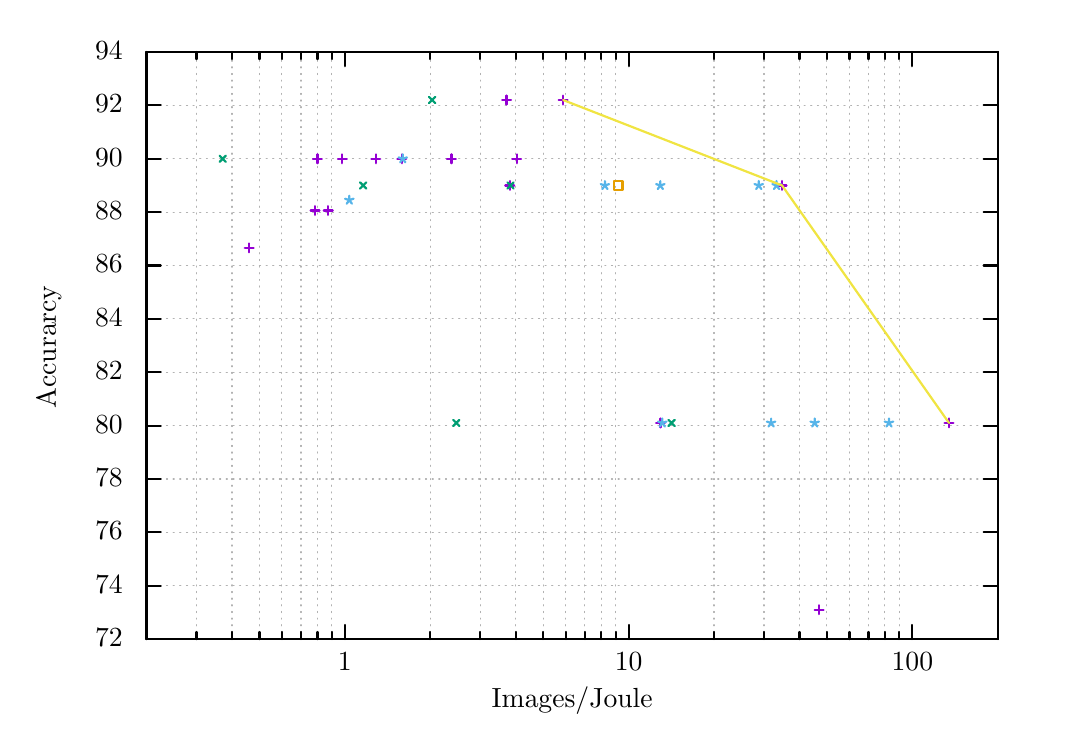
\begin{tikzpicture}[gnuplot]
%% generated with GNUPLOT 5.2p2 (Lua 5.3; terminal rev. 99, script rev. 102)
%% Di 18 Dez 2018 07:15:13 CET
\path (0.000,0.000) rectangle (12.500,8.750);
\gpcolor{color=gp lt color axes}
\gpsetlinetype{gp lt axes}
\gpsetdashtype{gp dt axes}
\gpsetlinewidth{1.00}
\draw[gp path] (1.136,0.985)--(11.947,0.985);
\gpcolor{color=gp lt color border}
\gpsetlinetype{gp lt border}
\gpsetdashtype{gp dt solid}
\gpsetlinewidth{2.00}
\draw[gp path] (1.136,0.985)--(1.316,0.985);
\draw[gp path] (11.947,0.985)--(11.767,0.985);
\node[gp node right] at (0.952,0.985) {$72$};
\gpcolor{color=gp lt color axes}
\gpsetlinetype{gp lt axes}
\gpsetdashtype{gp dt axes}
\gpsetlinewidth{1.00}
\draw[gp path] (1.136,1.663)--(11.947,1.663);
\gpcolor{color=gp lt color border}
\gpsetlinetype{gp lt border}
\gpsetdashtype{gp dt solid}
\gpsetlinewidth{2.00}
\draw[gp path] (1.136,1.663)--(1.316,1.663);
\draw[gp path] (11.947,1.663)--(11.767,1.663);
\node[gp node right] at (0.952,1.663) {$74$};
\gpcolor{color=gp lt color axes}
\gpsetlinetype{gp lt axes}
\gpsetdashtype{gp dt axes}
\gpsetlinewidth{1.00}
\draw[gp path] (1.136,2.341)--(11.947,2.341);
\gpcolor{color=gp lt color border}
\gpsetlinetype{gp lt border}
\gpsetdashtype{gp dt solid}
\gpsetlinewidth{2.00}
\draw[gp path] (1.136,2.341)--(1.316,2.341);
\draw[gp path] (11.947,2.341)--(11.767,2.341);
\node[gp node right] at (0.952,2.341) {$76$};
\gpcolor{color=gp lt color axes}
\gpsetlinetype{gp lt axes}
\gpsetdashtype{gp dt axes}
\gpsetlinewidth{1.00}
\draw[gp path] (1.136,3.018)--(11.947,3.018);
\gpcolor{color=gp lt color border}
\gpsetlinetype{gp lt border}
\gpsetdashtype{gp dt solid}
\gpsetlinewidth{2.00}
\draw[gp path] (1.136,3.018)--(1.316,3.018);
\draw[gp path] (11.947,3.018)--(11.767,3.018);
\node[gp node right] at (0.952,3.018) {$78$};
\gpcolor{color=gp lt color axes}
\gpsetlinetype{gp lt axes}
\gpsetdashtype{gp dt axes}
\gpsetlinewidth{1.00}
\draw[gp path] (1.136,3.696)--(11.947,3.696);
\gpcolor{color=gp lt color border}
\gpsetlinetype{gp lt border}
\gpsetdashtype{gp dt solid}
\gpsetlinewidth{2.00}
\draw[gp path] (1.136,3.696)--(1.316,3.696);
\draw[gp path] (11.947,3.696)--(11.767,3.696);
\node[gp node right] at (0.952,3.696) {$80$};
\gpcolor{color=gp lt color axes}
\gpsetlinetype{gp lt axes}
\gpsetdashtype{gp dt axes}
\gpsetlinewidth{1.00}
\draw[gp path] (1.136,4.374)--(11.947,4.374);
\gpcolor{color=gp lt color border}
\gpsetlinetype{gp lt border}
\gpsetdashtype{gp dt solid}
\gpsetlinewidth{2.00}
\draw[gp path] (1.136,4.374)--(1.316,4.374);
\draw[gp path] (11.947,4.374)--(11.767,4.374);
\node[gp node right] at (0.952,4.374) {$82$};
\gpcolor{color=gp lt color axes}
\gpsetlinetype{gp lt axes}
\gpsetdashtype{gp dt axes}
\gpsetlinewidth{1.00}
\draw[gp path] (1.136,5.052)--(11.947,5.052);
\gpcolor{color=gp lt color border}
\gpsetlinetype{gp lt border}
\gpsetdashtype{gp dt solid}
\gpsetlinewidth{2.00}
\draw[gp path] (1.136,5.052)--(1.316,5.052);
\draw[gp path] (11.947,5.052)--(11.767,5.052);
\node[gp node right] at (0.952,5.052) {$84$};
\gpcolor{color=gp lt color axes}
\gpsetlinetype{gp lt axes}
\gpsetdashtype{gp dt axes}
\gpsetlinewidth{1.00}
\draw[gp path] (1.136,5.730)--(11.947,5.730);
\gpcolor{color=gp lt color border}
\gpsetlinetype{gp lt border}
\gpsetdashtype{gp dt solid}
\gpsetlinewidth{2.00}
\draw[gp path] (1.136,5.730)--(1.316,5.730);
\draw[gp path] (11.947,5.730)--(11.767,5.730);
\node[gp node right] at (0.952,5.730) {$86$};
\gpcolor{color=gp lt color axes}
\gpsetlinetype{gp lt axes}
\gpsetdashtype{gp dt axes}
\gpsetlinewidth{1.00}
\draw[gp path] (1.136,6.408)--(11.947,6.408);
\gpcolor{color=gp lt color border}
\gpsetlinetype{gp lt border}
\gpsetdashtype{gp dt solid}
\gpsetlinewidth{2.00}
\draw[gp path] (1.136,6.408)--(1.316,6.408);
\draw[gp path] (11.947,6.408)--(11.767,6.408);
\node[gp node right] at (0.952,6.408) {$88$};
\gpcolor{color=gp lt color axes}
\gpsetlinetype{gp lt axes}
\gpsetdashtype{gp dt axes}
\gpsetlinewidth{1.00}
\draw[gp path] (1.136,7.085)--(11.947,7.085);
\gpcolor{color=gp lt color border}
\gpsetlinetype{gp lt border}
\gpsetdashtype{gp dt solid}
\gpsetlinewidth{2.00}
\draw[gp path] (1.136,7.085)--(1.316,7.085);
\draw[gp path] (11.947,7.085)--(11.767,7.085);
\node[gp node right] at (0.952,7.085) {$90$};
\gpcolor{color=gp lt color axes}
\gpsetlinetype{gp lt axes}
\gpsetdashtype{gp dt axes}
\gpsetlinewidth{1.00}
\draw[gp path] (1.136,7.763)--(11.947,7.763);
\gpcolor{color=gp lt color border}
\gpsetlinetype{gp lt border}
\gpsetdashtype{gp dt solid}
\gpsetlinewidth{2.00}
\draw[gp path] (1.136,7.763)--(1.316,7.763);
\draw[gp path] (11.947,7.763)--(11.767,7.763);
\node[gp node right] at (0.952,7.763) {$92$};
\gpcolor{color=gp lt color axes}
\gpsetlinetype{gp lt axes}
\gpsetdashtype{gp dt axes}
\gpsetlinewidth{1.00}
\draw[gp path] (1.136,8.441)--(11.947,8.441);
\gpcolor{color=gp lt color border}
\gpsetlinetype{gp lt border}
\gpsetdashtype{gp dt solid}
\gpsetlinewidth{2.00}
\draw[gp path] (1.136,8.441)--(1.316,8.441);
\draw[gp path] (11.947,8.441)--(11.767,8.441);
\node[gp node right] at (0.952,8.441) {$94$};
\gpcolor{color=gp lt color axes}
\gpsetlinetype{gp lt axes}
\gpsetdashtype{gp dt axes}
\gpsetlinewidth{1.00}
\draw[gp path] (1.136,0.985)--(1.136,8.441);
\gpcolor{color=gp lt color border}
\gpsetlinetype{gp lt border}
\gpsetdashtype{gp dt solid}
\gpsetlinewidth{2.00}
\draw[gp path] (1.136,0.985)--(1.136,1.075);
\draw[gp path] (1.136,8.441)--(1.136,8.351);
\gpcolor{color=gp lt color axes}
\gpsetlinetype{gp lt axes}
\gpsetdashtype{gp dt axes}
\gpsetlinewidth{1.00}
\draw[gp path] (1.771,0.985)--(1.771,8.441);
\gpcolor{color=gp lt color border}
\gpsetlinetype{gp lt border}
\gpsetdashtype{gp dt solid}
\gpsetlinewidth{2.00}
\draw[gp path] (1.771,0.985)--(1.771,1.075);
\draw[gp path] (1.771,8.441)--(1.771,8.351);
\gpcolor{color=gp lt color axes}
\gpsetlinetype{gp lt axes}
\gpsetdashtype{gp dt axes}
\gpsetlinewidth{1.00}
\draw[gp path] (2.221,0.985)--(2.221,8.441);
\gpcolor{color=gp lt color border}
\gpsetlinetype{gp lt border}
\gpsetdashtype{gp dt solid}
\gpsetlinewidth{2.00}
\draw[gp path] (2.221,0.985)--(2.221,1.075);
\draw[gp path] (2.221,8.441)--(2.221,8.351);
\gpcolor{color=gp lt color axes}
\gpsetlinetype{gp lt axes}
\gpsetdashtype{gp dt axes}
\gpsetlinewidth{1.00}
\draw[gp path] (2.570,0.985)--(2.570,8.441);
\gpcolor{color=gp lt color border}
\gpsetlinetype{gp lt border}
\gpsetdashtype{gp dt solid}
\gpsetlinewidth{2.00}
\draw[gp path] (2.570,0.985)--(2.570,1.075);
\draw[gp path] (2.570,8.441)--(2.570,8.351);
\gpcolor{color=gp lt color axes}
\gpsetlinetype{gp lt axes}
\gpsetdashtype{gp dt axes}
\gpsetlinewidth{1.00}
\draw[gp path] (2.855,0.985)--(2.855,8.441);
\gpcolor{color=gp lt color border}
\gpsetlinetype{gp lt border}
\gpsetdashtype{gp dt solid}
\gpsetlinewidth{2.00}
\draw[gp path] (2.855,0.985)--(2.855,1.075);
\draw[gp path] (2.855,8.441)--(2.855,8.351);
\gpcolor{color=gp lt color axes}
\gpsetlinetype{gp lt axes}
\gpsetdashtype{gp dt axes}
\gpsetlinewidth{1.00}
\draw[gp path] (3.097,0.985)--(3.097,8.441);
\gpcolor{color=gp lt color border}
\gpsetlinetype{gp lt border}
\gpsetdashtype{gp dt solid}
\gpsetlinewidth{2.00}
\draw[gp path] (3.097,0.985)--(3.097,1.075);
\draw[gp path] (3.097,8.441)--(3.097,8.351);
\gpcolor{color=gp lt color axes}
\gpsetlinetype{gp lt axes}
\gpsetdashtype{gp dt axes}
\gpsetlinewidth{1.00}
\draw[gp path] (3.306,0.985)--(3.306,8.441);
\gpcolor{color=gp lt color border}
\gpsetlinetype{gp lt border}
\gpsetdashtype{gp dt solid}
\gpsetlinewidth{2.00}
\draw[gp path] (3.306,0.985)--(3.306,1.075);
\draw[gp path] (3.306,8.441)--(3.306,8.351);
\gpcolor{color=gp lt color axes}
\gpsetlinetype{gp lt axes}
\gpsetdashtype{gp dt axes}
\gpsetlinewidth{1.00}
\draw[gp path] (3.490,0.985)--(3.490,8.441);
\gpcolor{color=gp lt color border}
\gpsetlinetype{gp lt border}
\gpsetdashtype{gp dt solid}
\gpsetlinewidth{2.00}
\draw[gp path] (3.490,0.985)--(3.490,1.075);
\draw[gp path] (3.490,8.441)--(3.490,8.351);
\draw[gp path] (3.655,0.985)--(3.655,1.165);
\draw[gp path] (3.655,8.441)--(3.655,8.261);
\node[gp node center] at (3.655,0.677) {$1$};
\gpcolor{color=gp lt color axes}
\gpsetlinetype{gp lt axes}
\gpsetdashtype{gp dt axes}
\gpsetlinewidth{1.00}
\draw[gp path] (4.740,0.985)--(4.740,8.441);
\gpcolor{color=gp lt color border}
\gpsetlinetype{gp lt border}
\gpsetdashtype{gp dt solid}
\gpsetlinewidth{2.00}
\draw[gp path] (4.740,0.985)--(4.740,1.075);
\draw[gp path] (4.740,8.441)--(4.740,8.351);
\gpcolor{color=gp lt color axes}
\gpsetlinetype{gp lt axes}
\gpsetdashtype{gp dt axes}
\gpsetlinewidth{1.00}
\draw[gp path] (5.374,0.985)--(5.374,8.441);
\gpcolor{color=gp lt color border}
\gpsetlinetype{gp lt border}
\gpsetdashtype{gp dt solid}
\gpsetlinewidth{2.00}
\draw[gp path] (5.374,0.985)--(5.374,1.075);
\draw[gp path] (5.374,8.441)--(5.374,8.351);
\gpcolor{color=gp lt color axes}
\gpsetlinetype{gp lt axes}
\gpsetdashtype{gp dt axes}
\gpsetlinewidth{1.00}
\draw[gp path] (5.824,0.985)--(5.824,8.441);
\gpcolor{color=gp lt color border}
\gpsetlinetype{gp lt border}
\gpsetdashtype{gp dt solid}
\gpsetlinewidth{2.00}
\draw[gp path] (5.824,0.985)--(5.824,1.075);
\draw[gp path] (5.824,8.441)--(5.824,8.351);
\gpcolor{color=gp lt color axes}
\gpsetlinetype{gp lt axes}
\gpsetdashtype{gp dt axes}
\gpsetlinewidth{1.00}
\draw[gp path] (6.174,0.985)--(6.174,8.441);
\gpcolor{color=gp lt color border}
\gpsetlinetype{gp lt border}
\gpsetdashtype{gp dt solid}
\gpsetlinewidth{2.00}
\draw[gp path] (6.174,0.985)--(6.174,1.075);
\draw[gp path] (6.174,8.441)--(6.174,8.351);
\gpcolor{color=gp lt color axes}
\gpsetlinetype{gp lt axes}
\gpsetdashtype{gp dt axes}
\gpsetlinewidth{1.00}
\draw[gp path] (6.459,0.985)--(6.459,8.441);
\gpcolor{color=gp lt color border}
\gpsetlinetype{gp lt border}
\gpsetdashtype{gp dt solid}
\gpsetlinewidth{2.00}
\draw[gp path] (6.459,0.985)--(6.459,1.075);
\draw[gp path] (6.459,8.441)--(6.459,8.351);
\gpcolor{color=gp lt color axes}
\gpsetlinetype{gp lt axes}
\gpsetdashtype{gp dt axes}
\gpsetlinewidth{1.00}
\draw[gp path] (6.700,0.985)--(6.700,8.441);
\gpcolor{color=gp lt color border}
\gpsetlinetype{gp lt border}
\gpsetdashtype{gp dt solid}
\gpsetlinewidth{2.00}
\draw[gp path] (6.700,0.985)--(6.700,1.075);
\draw[gp path] (6.700,8.441)--(6.700,8.351);
\gpcolor{color=gp lt color axes}
\gpsetlinetype{gp lt axes}
\gpsetdashtype{gp dt axes}
\gpsetlinewidth{1.00}
\draw[gp path] (6.909,0.985)--(6.909,8.441);
\gpcolor{color=gp lt color border}
\gpsetlinetype{gp lt border}
\gpsetdashtype{gp dt solid}
\gpsetlinewidth{2.00}
\draw[gp path] (6.909,0.985)--(6.909,1.075);
\draw[gp path] (6.909,8.441)--(6.909,8.351);
\gpcolor{color=gp lt color axes}
\gpsetlinetype{gp lt axes}
\gpsetdashtype{gp dt axes}
\gpsetlinewidth{1.00}
\draw[gp path] (7.094,0.985)--(7.094,8.441);
\gpcolor{color=gp lt color border}
\gpsetlinetype{gp lt border}
\gpsetdashtype{gp dt solid}
\gpsetlinewidth{2.00}
\draw[gp path] (7.094,0.985)--(7.094,1.075);
\draw[gp path] (7.094,8.441)--(7.094,8.351);
\draw[gp path] (7.259,0.985)--(7.259,1.165);
\draw[gp path] (7.259,8.441)--(7.259,8.261);
\node[gp node center] at (7.259,0.677) {$10$};
\gpcolor{color=gp lt color axes}
\gpsetlinetype{gp lt axes}
\gpsetdashtype{gp dt axes}
\gpsetlinewidth{1.00}
\draw[gp path] (8.343,0.985)--(8.343,8.441);
\gpcolor{color=gp lt color border}
\gpsetlinetype{gp lt border}
\gpsetdashtype{gp dt solid}
\gpsetlinewidth{2.00}
\draw[gp path] (8.343,0.985)--(8.343,1.075);
\draw[gp path] (8.343,8.441)--(8.343,8.351);
\gpcolor{color=gp lt color axes}
\gpsetlinetype{gp lt axes}
\gpsetdashtype{gp dt axes}
\gpsetlinewidth{1.00}
\draw[gp path] (8.978,0.985)--(8.978,8.441);
\gpcolor{color=gp lt color border}
\gpsetlinetype{gp lt border}
\gpsetdashtype{gp dt solid}
\gpsetlinewidth{2.00}
\draw[gp path] (8.978,0.985)--(8.978,1.075);
\draw[gp path] (8.978,8.441)--(8.978,8.351);
\gpcolor{color=gp lt color axes}
\gpsetlinetype{gp lt axes}
\gpsetdashtype{gp dt axes}
\gpsetlinewidth{1.00}
\draw[gp path] (9.428,0.985)--(9.428,8.441);
\gpcolor{color=gp lt color border}
\gpsetlinetype{gp lt border}
\gpsetdashtype{gp dt solid}
\gpsetlinewidth{2.00}
\draw[gp path] (9.428,0.985)--(9.428,1.075);
\draw[gp path] (9.428,8.441)--(9.428,8.351);
\gpcolor{color=gp lt color axes}
\gpsetlinetype{gp lt axes}
\gpsetdashtype{gp dt axes}
\gpsetlinewidth{1.00}
\draw[gp path] (9.777,0.985)--(9.777,8.441);
\gpcolor{color=gp lt color border}
\gpsetlinetype{gp lt border}
\gpsetdashtype{gp dt solid}
\gpsetlinewidth{2.00}
\draw[gp path] (9.777,0.985)--(9.777,1.075);
\draw[gp path] (9.777,8.441)--(9.777,8.351);
\gpcolor{color=gp lt color axes}
\gpsetlinetype{gp lt axes}
\gpsetdashtype{gp dt axes}
\gpsetlinewidth{1.00}
\draw[gp path] (10.063,0.985)--(10.063,8.441);
\gpcolor{color=gp lt color border}
\gpsetlinetype{gp lt border}
\gpsetdashtype{gp dt solid}
\gpsetlinewidth{2.00}
\draw[gp path] (10.063,0.985)--(10.063,1.075);
\draw[gp path] (10.063,8.441)--(10.063,8.351);
\gpcolor{color=gp lt color axes}
\gpsetlinetype{gp lt axes}
\gpsetdashtype{gp dt axes}
\gpsetlinewidth{1.00}
\draw[gp path] (10.304,0.985)--(10.304,8.441);
\gpcolor{color=gp lt color border}
\gpsetlinetype{gp lt border}
\gpsetdashtype{gp dt solid}
\gpsetlinewidth{2.00}
\draw[gp path] (10.304,0.985)--(10.304,1.075);
\draw[gp path] (10.304,8.441)--(10.304,8.351);
\gpcolor{color=gp lt color axes}
\gpsetlinetype{gp lt axes}
\gpsetdashtype{gp dt axes}
\gpsetlinewidth{1.00}
\draw[gp path] (10.513,0.985)--(10.513,8.261)--(10.513,8.441);
\gpcolor{color=gp lt color border}
\gpsetlinetype{gp lt border}
\gpsetdashtype{gp dt solid}
\gpsetlinewidth{2.00}
\draw[gp path] (10.513,0.985)--(10.513,1.075);
\draw[gp path] (10.513,8.441)--(10.513,8.351);
\gpcolor{color=gp lt color axes}
\gpsetlinetype{gp lt axes}
\gpsetdashtype{gp dt axes}
\gpsetlinewidth{1.00}
\draw[gp path] (10.697,0.985)--(10.697,8.261)--(10.697,8.441);
\gpcolor{color=gp lt color border}
\gpsetlinetype{gp lt border}
\gpsetdashtype{gp dt solid}
\gpsetlinewidth{2.00}
\draw[gp path] (10.697,0.985)--(10.697,1.075);
\draw[gp path] (10.697,8.441)--(10.697,8.351);
\draw[gp path] (10.862,0.985)--(10.862,1.165);
\draw[gp path] (10.862,8.441)--(10.862,8.261);
\node[gp node center] at (10.862,0.677) {$100$};
\gpcolor{color=gp lt color axes}
\gpsetlinetype{gp lt axes}
\gpsetdashtype{gp dt axes}
\gpsetlinewidth{1.00}
\draw[gp path] (11.947,0.985)--(11.947,8.441);
\gpcolor{color=gp lt color border}
\gpsetlinetype{gp lt border}
\gpsetdashtype{gp dt solid}
\gpsetlinewidth{2.00}
\draw[gp path] (11.947,0.985)--(11.947,1.075);
\draw[gp path] (11.947,8.441)--(11.947,8.351);
\draw[gp path] (1.136,8.441)--(1.136,0.985)--(11.947,0.985)--(11.947,8.441)--cycle;
\node[gp node center,rotate=-270] at (-0.092,4.713) {Accurarcy};
\node[gp node center] at (6.541,0.215) {Images/Joule};
\gpcolor{rgb color={0.580,0.000,0.827}}
\gpsetpointsize{4.00}
\gppoint{gp mark 1}{(9.677,1.358)}
\gppoint{gp mark 1}{(5.837,7.085)}
\gppoint{gp mark 1}{(2.440,5.953)}
\gppoint{gp mark 1}{(7.663,3.730)}
\gppoint{gp mark 1}{(3.623,7.085)}
\gppoint{gp mark 1}{(5.708,7.831)}
\gppoint{gp mark 1}{(3.444,6.428)}
\gppoint{gp mark 1}{(5.008,7.085)}
\gppoint{gp mark 1}{(3.276,6.428)}
\gppoint{gp mark 1}{(3.306,7.085)}
\gppoint{gp mark 1}{(5.748,6.746)}
\gppoint{gp mark 1}{(6.427,7.831)}
\gppoint{gp mark 1}{(11.327,3.730)}
\gppoint{gp mark 1}{(4.047,7.085)}
\gppoint{gp mark 1}{(4.377,7.085)}
\gppoint{gp mark 1}{(9.207,6.746)}
\gpcolor{rgb color={0.000,0.620,0.451}}
\gppoint{gp mark 2}{(5.070,3.730)}
\gppoint{gp mark 2}{(7.804,3.730)}
\gppoint{gp mark 2}{(2.103,7.085)}
\gppoint{gp mark 2}{(3.887,6.746)}
\gppoint{gp mark 2}{(5.759,6.746)}
\gppoint{gp mark 2}{(4.763,7.831)}
\gpcolor{rgb color={0.337,0.706,0.914}}
\gppoint{gp mark 3}{(3.711,6.560)}
\gppoint{gp mark 3}{(7.686,3.730)}
\gppoint{gp mark 3}{(9.622,3.730)}
\gppoint{gp mark 3}{(9.068,3.730)}
\gppoint{gp mark 3}{(10.565,3.730)}
\gppoint{gp mark 3}{(6.957,6.746)}
\gppoint{gp mark 3}{(7.661,6.746)}
\gppoint{gp mark 3}{(8.911,6.746)}
\gppoint{gp mark 3}{(9.137,6.746)}
\gppoint{gp mark 3}{(4.390,7.085)}
\gpcolor{rgb color={0.902,0.624,0.000}}
\gppoint{gp mark 4}{(7.124,6.746)}
\gpcolor{rgb color={0.941,0.894,0.259}}
\draw[gp path] (6.427,7.831)--(9.207,6.746)--(11.327,3.730);
\gpcolor{color=gp lt color border}
\draw[gp path] (1.136,8.441)--(1.136,0.985)--(11.947,0.985)--(11.947,8.441)--cycle;
%% coordinates of the plot area
\gpdefrectangularnode{gp plot 1}{\pgfpoint{1.136cm}{0.985cm}}{\pgfpoint{11.947cm}{8.441cm}}
\end{tikzpicture}
%% gnuplot variables
}
    \hfill
    \scalebox{0.8}{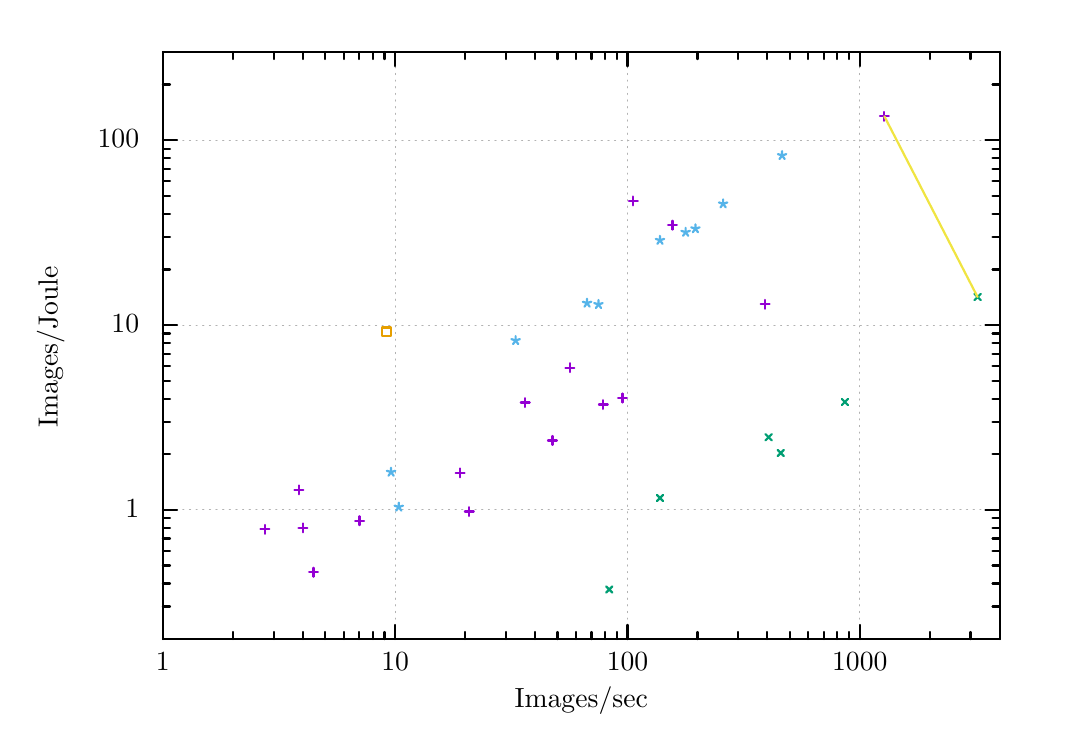
\begin{tikzpicture}[gnuplot]
%% generated with GNUPLOT 5.2p2 (Lua 5.3; terminal rev. 99, script rev. 102)
%% Di 18 Dez 2018 07:44:18 CET
\path (0.000,0.000) rectangle (12.500,8.750);
\gpcolor{color=gp lt color border}
\gpsetlinetype{gp lt border}
\gpsetdashtype{gp dt solid}
\gpsetlinewidth{2.00}
\draw[gp path] (1.320,0.985)--(1.410,0.985);
\draw[gp path] (11.947,0.985)--(11.857,0.985);
\draw[gp path] (1.320,1.398)--(1.410,1.398);
\draw[gp path] (11.947,1.398)--(11.857,1.398);
\draw[gp path] (1.320,1.692)--(1.410,1.692);
\draw[gp path] (11.947,1.692)--(11.857,1.692);
\draw[gp path] (1.320,1.919)--(1.410,1.919);
\draw[gp path] (11.947,1.919)--(11.857,1.919);
\draw[gp path] (1.320,2.105)--(1.410,2.105);
\draw[gp path] (11.947,2.105)--(11.857,2.105);
\draw[gp path] (1.320,2.262)--(1.410,2.262);
\draw[gp path] (11.947,2.262)--(11.857,2.262);
\draw[gp path] (1.320,2.398)--(1.410,2.398);
\draw[gp path] (11.947,2.398)--(11.857,2.398);
\draw[gp path] (1.320,2.518)--(1.410,2.518);
\draw[gp path] (11.947,2.518)--(11.857,2.518);
\gpcolor{color=gp lt color axes}
\gpsetlinetype{gp lt axes}
\gpsetdashtype{gp dt axes}
\gpsetlinewidth{1.00}
\draw[gp path] (1.320,2.626)--(11.947,2.626);
\gpcolor{color=gp lt color border}
\gpsetlinetype{gp lt border}
\gpsetdashtype{gp dt solid}
\gpsetlinewidth{2.00}
\draw[gp path] (1.320,2.626)--(1.500,2.626);
\draw[gp path] (11.947,2.626)--(11.767,2.626);
\node[gp node right] at (1.136,2.626) {$1$};
\draw[gp path] (1.320,3.333)--(1.410,3.333);
\draw[gp path] (11.947,3.333)--(11.857,3.333);
\draw[gp path] (1.320,3.746)--(1.410,3.746);
\draw[gp path] (11.947,3.746)--(11.857,3.746);
\draw[gp path] (1.320,4.039)--(1.410,4.039);
\draw[gp path] (11.947,4.039)--(11.857,4.039);
\draw[gp path] (1.320,4.267)--(1.410,4.267);
\draw[gp path] (11.947,4.267)--(11.857,4.267);
\draw[gp path] (1.320,4.453)--(1.410,4.453);
\draw[gp path] (11.947,4.453)--(11.857,4.453);
\draw[gp path] (1.320,4.610)--(1.410,4.610);
\draw[gp path] (11.947,4.610)--(11.857,4.610);
\draw[gp path] (1.320,4.746)--(1.410,4.746);
\draw[gp path] (11.947,4.746)--(11.857,4.746);
\draw[gp path] (1.320,4.866)--(1.410,4.866);
\draw[gp path] (11.947,4.866)--(11.857,4.866);
\gpcolor{color=gp lt color axes}
\gpsetlinetype{gp lt axes}
\gpsetdashtype{gp dt axes}
\gpsetlinewidth{1.00}
\draw[gp path] (1.320,4.973)--(11.947,4.973);
\gpcolor{color=gp lt color border}
\gpsetlinetype{gp lt border}
\gpsetdashtype{gp dt solid}
\gpsetlinewidth{2.00}
\draw[gp path] (1.320,4.973)--(1.500,4.973);
\draw[gp path] (11.947,4.973)--(11.767,4.973);
\node[gp node right] at (1.136,4.973) {$10$};
\draw[gp path] (1.320,5.680)--(1.410,5.680);
\draw[gp path] (11.947,5.680)--(11.857,5.680);
\draw[gp path] (1.320,6.093)--(1.410,6.093);
\draw[gp path] (11.947,6.093)--(11.857,6.093);
\draw[gp path] (1.320,6.387)--(1.410,6.387);
\draw[gp path] (11.947,6.387)--(11.857,6.387);
\draw[gp path] (1.320,6.614)--(1.410,6.614);
\draw[gp path] (11.947,6.614)--(11.857,6.614);
\draw[gp path] (1.320,6.800)--(1.410,6.800);
\draw[gp path] (11.947,6.800)--(11.857,6.800);
\draw[gp path] (1.320,6.957)--(1.410,6.957);
\draw[gp path] (11.947,6.957)--(11.857,6.957);
\draw[gp path] (1.320,7.093)--(1.410,7.093);
\draw[gp path] (11.947,7.093)--(11.857,7.093);
\draw[gp path] (1.320,7.214)--(1.410,7.214);
\draw[gp path] (11.947,7.214)--(11.857,7.214);
\gpcolor{color=gp lt color axes}
\gpsetlinetype{gp lt axes}
\gpsetdashtype{gp dt axes}
\gpsetlinewidth{1.00}
\draw[gp path] (1.320,7.321)--(11.947,7.321);
\gpcolor{color=gp lt color border}
\gpsetlinetype{gp lt border}
\gpsetdashtype{gp dt solid}
\gpsetlinewidth{2.00}
\draw[gp path] (1.320,7.321)--(1.500,7.321);
\draw[gp path] (11.947,7.321)--(11.767,7.321);
\node[gp node right] at (1.136,7.321) {$100$};
\draw[gp path] (1.320,8.028)--(1.410,8.028);
\draw[gp path] (11.947,8.028)--(11.857,8.028);
\draw[gp path] (1.320,8.441)--(1.410,8.441);
\draw[gp path] (11.947,8.441)--(11.857,8.441);
\gpcolor{color=gp lt color axes}
\gpsetlinetype{gp lt axes}
\gpsetdashtype{gp dt axes}
\gpsetlinewidth{1.00}
\draw[gp path] (1.320,0.985)--(1.320,8.441);
\gpcolor{color=gp lt color border}
\gpsetlinetype{gp lt border}
\gpsetdashtype{gp dt solid}
\gpsetlinewidth{2.00}
\draw[gp path] (1.320,0.985)--(1.320,1.165);
\draw[gp path] (1.320,8.441)--(1.320,8.261);
\node[gp node center] at (1.320,0.677) {$1$};
\draw[gp path] (2.208,0.985)--(2.208,1.075);
\draw[gp path] (2.208,8.441)--(2.208,8.351);
\draw[gp path] (2.728,0.985)--(2.728,1.075);
\draw[gp path] (2.728,8.441)--(2.728,8.351);
\draw[gp path] (3.096,0.985)--(3.096,1.075);
\draw[gp path] (3.096,8.441)--(3.096,8.351);
\draw[gp path] (3.382,0.985)--(3.382,1.075);
\draw[gp path] (3.382,8.441)--(3.382,8.351);
\draw[gp path] (3.616,0.985)--(3.616,1.075);
\draw[gp path] (3.616,8.441)--(3.616,8.351);
\draw[gp path] (3.813,0.985)--(3.813,1.075);
\draw[gp path] (3.813,8.441)--(3.813,8.351);
\draw[gp path] (3.984,0.985)--(3.984,1.075);
\draw[gp path] (3.984,8.441)--(3.984,8.351);
\draw[gp path] (4.135,0.985)--(4.135,1.075);
\draw[gp path] (4.135,8.441)--(4.135,8.351);
\gpcolor{color=gp lt color axes}
\gpsetlinetype{gp lt axes}
\gpsetdashtype{gp dt axes}
\gpsetlinewidth{1.00}
\draw[gp path] (4.270,0.985)--(4.270,8.441);
\gpcolor{color=gp lt color border}
\gpsetlinetype{gp lt border}
\gpsetdashtype{gp dt solid}
\gpsetlinewidth{2.00}
\draw[gp path] (4.270,0.985)--(4.270,1.165);
\draw[gp path] (4.270,8.441)--(4.270,8.261);
\node[gp node center] at (4.270,0.677) {$10$};
\draw[gp path] (5.158,0.985)--(5.158,1.075);
\draw[gp path] (5.158,8.441)--(5.158,8.351);
\draw[gp path] (5.678,0.985)--(5.678,1.075);
\draw[gp path] (5.678,8.441)--(5.678,8.351);
\draw[gp path] (6.046,0.985)--(6.046,1.075);
\draw[gp path] (6.046,8.441)--(6.046,8.351);
\draw[gp path] (6.332,0.985)--(6.332,1.075);
\draw[gp path] (6.332,8.441)--(6.332,8.351);
\draw[gp path] (6.566,0.985)--(6.566,1.075);
\draw[gp path] (6.566,8.441)--(6.566,8.351);
\draw[gp path] (6.764,0.985)--(6.764,1.075);
\draw[gp path] (6.764,8.441)--(6.764,8.351);
\draw[gp path] (6.935,0.985)--(6.935,1.075);
\draw[gp path] (6.935,8.441)--(6.935,8.351);
\draw[gp path] (7.086,0.985)--(7.086,1.075);
\draw[gp path] (7.086,8.441)--(7.086,8.351);
\gpcolor{color=gp lt color axes}
\gpsetlinetype{gp lt axes}
\gpsetdashtype{gp dt axes}
\gpsetlinewidth{1.00}
\draw[gp path] (7.221,0.985)--(7.221,8.441);
\gpcolor{color=gp lt color border}
\gpsetlinetype{gp lt border}
\gpsetdashtype{gp dt solid}
\gpsetlinewidth{2.00}
\draw[gp path] (7.221,0.985)--(7.221,1.165);
\draw[gp path] (7.221,8.441)--(7.221,8.261);
\node[gp node center] at (7.221,0.677) {$100$};
\draw[gp path] (8.109,0.985)--(8.109,1.075);
\draw[gp path] (8.109,8.441)--(8.109,8.351);
\draw[gp path] (8.628,0.985)--(8.628,1.075);
\draw[gp path] (8.628,8.441)--(8.628,8.351);
\draw[gp path] (8.997,0.985)--(8.997,1.075);
\draw[gp path] (8.997,8.441)--(8.997,8.351);
\draw[gp path] (9.283,0.985)--(9.283,1.075);
\draw[gp path] (9.283,8.441)--(9.283,8.351);
\draw[gp path] (9.516,0.985)--(9.516,1.075);
\draw[gp path] (9.516,8.441)--(9.516,8.351);
\draw[gp path] (9.714,0.985)--(9.714,1.075);
\draw[gp path] (9.714,8.441)--(9.714,8.351);
\draw[gp path] (9.885,0.985)--(9.885,1.075);
\draw[gp path] (9.885,8.441)--(9.885,8.351);
\draw[gp path] (10.036,0.985)--(10.036,1.075);
\draw[gp path] (10.036,8.441)--(10.036,8.351);
\gpcolor{color=gp lt color axes}
\gpsetlinetype{gp lt axes}
\gpsetdashtype{gp dt axes}
\gpsetlinewidth{1.00}
\draw[gp path] (10.171,0.985)--(10.171,8.441);
\gpcolor{color=gp lt color border}
\gpsetlinetype{gp lt border}
\gpsetdashtype{gp dt solid}
\gpsetlinewidth{2.00}
\draw[gp path] (10.171,0.985)--(10.171,1.165);
\draw[gp path] (10.171,8.441)--(10.171,8.261);
\node[gp node center] at (10.171,0.677) {$1000$};
\draw[gp path] (11.059,0.985)--(11.059,1.075);
\draw[gp path] (11.059,8.441)--(11.059,8.351);
\draw[gp path] (11.578,0.985)--(11.578,1.075);
\draw[gp path] (11.578,8.441)--(11.578,8.351);
\draw[gp path] (11.947,0.985)--(11.947,1.075);
\draw[gp path] (11.947,8.441)--(11.947,8.351);
\draw[gp path] (1.320,8.441)--(1.320,0.985)--(11.947,0.985)--(11.947,8.441)--cycle;
\node[gp node center,rotate=-270] at (-0.092,4.713) {Images/Joule};
\node[gp node center] at (6.633,0.215) {Images/sec};
\gpcolor{rgb color={0.580,0.000,0.827}}
\gpsetpointsize{4.00}
\gppoint{gp mark 1}{(7.295,6.549)}
\gppoint{gp mark 1}{(7.157,4.047)}
\gppoint{gp mark 1}{(3.233,1.834)}
\gppoint{gp mark 1}{(8.968,5.237)}
\gppoint{gp mark 1}{(5.212,2.605)}
\gppoint{gp mark 1}{(6.914,3.964)}
\gppoint{gp mark 1}{(3.818,2.489)}
\gppoint{gp mark 1}{(6.267,3.508)}
\gppoint{gp mark 1}{(2.615,2.379)}
\gppoint{gp mark 1}{(3.099,2.398)}
\gppoint{gp mark 1}{(5.922,3.989)}
\gppoint{gp mark 1}{(6.489,4.432)}
\gppoint{gp mark 1}{(10.483,7.624)}
\gppoint{gp mark 1}{(3.048,2.881)}
\gppoint{gp mark 1}{(5.095,3.096)}
\gppoint{gp mark 1}{(7.792,6.242)}
\gpcolor{rgb color={0.000,0.620,0.451}}
\gppoint{gp mark 2}{(9.013,3.548)}
\gppoint{gp mark 2}{(11.667,5.329)}
\gppoint{gp mark 2}{(6.989,1.615)}
\gppoint{gp mark 2}{(7.633,2.777)}
\gppoint{gp mark 2}{(9.982,3.996)}
\gppoint{gp mark 2}{(9.167,3.348)}
\gpcolor{rgb color={0.337,0.706,0.914}}
\gppoint{gp mark 3}{(4.316,2.662)}
\gppoint{gp mark 3}{(6.707,5.252)}
\gppoint{gp mark 3}{(8.435,6.513)}
\gppoint{gp mark 3}{(7.959,6.152)}
\gppoint{gp mark 3}{(9.184,7.127)}
\gppoint{gp mark 3}{(5.800,4.777)}
\gppoint{gp mark 3}{(6.852,5.235)}
\gppoint{gp mark 3}{(7.633,6.050)}
\gppoint{gp mark 3}{(8.083,6.197)}
\gppoint{gp mark 3}{(4.218,3.105)}
\gpcolor{rgb color={0.902,0.624,0.000}}
\gppoint{gp mark 4}{(4.160,4.886)}
\gpcolor{rgb color={0.941,0.894,0.259}}
\draw[gp path] (10.483,7.624)--(11.667,5.329);
\gpcolor{color=gp lt color border}
\draw[gp path] (1.320,8.441)--(1.320,0.985)--(11.947,0.985)--(11.947,8.441)--cycle;
%% coordinates of the plot area
\gpdefrectangularnode{gp plot 1}{\pgfpoint{1.320cm}{0.985cm}}{\pgfpoint{11.947cm}{8.441cm}}
\end{tikzpicture}
%% gnuplot variables
}}
  \caption[]{Solutions for DNN implementations and evaluated with the
    ImageNet dataset as reported in recent publications from 2016-2018 and the
    Xilinx and Nvidia websites accessed in 2018.
    \label{fig:MW-Plots}}
\end{figure}


\end{document}
%
%----------------------------------------------------------------------------

%%% Local Variables:
%%% mode: latex
%%% TeX-master: t
%%% End:
